\chapter{Implementation Results and Delivered Platform}
\label{ch:platform}
\minitoc

\section*{Introduction}
\addcontentsline{toc}{section}{Introduction}

The preceding chapter closed with an agent that resolves a question and constructs a
verified answer. That agent is a library: it has no users, no memory, and no way of
reaching anyone who is not running Python on the same machine. This chapter presents the
platform built around it, and the order of presentation follows the order in which a
capability had to exist before the next one became possible.

The chapter opens with the architecture and the boundary that separates the immutable
knowledge base from mutable application state, since that boundary is what allowed every
subsequent feature to be added without touching the components responsible for
correctness. Access control follows, because an unauthenticated system cannot own a
conversation, and without ownership neither persistence nor sharing has any meaning. The
conversation interface and its input modes come next, then conversation persistence and
the sharing mechanism built on top of it. The dashboard is treated separately and at
length: it is the one part of the platform that reports on the matrix itself rather than
answering questions about it, and it turns out to expose properties of the document that
no page-by-page reading makes visible. The chapter closes with the REST surface, the test
suite, and deployment.

\section{Application Architecture}

Two structural decisions carry the rest of this chapter: how the client and server are
split, and how the two very different kinds of data the system holds are kept apart from
each other. Both were made early and never revisited, because later features were designed
to fit them rather than the other way round.

\subsection{Client--Server Structure}

The web client is a multi-page application rather than a single-page one. It is built with
React\citep{react_docs} and bundled by Vite\citep{vite_docs} into four independent entry
points, one each for the landing page, the sign-in page, the conversation page and the
dashboard, and the backend exposes a route for each that returns the corresponding
pre-built HTML document. The compiled JavaScript and stylesheet bundles are served from
two static mounts alongside them.

The distinction between what is written and what is served is worth making explicit, since
the two are not the same artefacts. The interface is authored as React components in JSX,
a syntax no browser can execute directly. The build step compiles that JSX into plain
JavaScript, bundles it, and emits for each entry point a minimal HTML document whose only
content is an empty mount element and a reference to the compiled bundle. What the backend
serves is therefore the compiled output, not the source: no JSX file exists in the deployed
artefact, and the interface a user sees is constructed in the browser by React once that
bundle has loaded and mounted into the empty element. Nothing is rendered or templated on the server: the
backend returns files that were produced at build time, and every dynamic element of a
page is populated by the client calling the API after it loads.

This was a deliberate choice rather than a simplification, and it trades a small amount of
navigation smoothness for two properties that matter more here. A single-page application
owns its own routing, which obliges the server to answer every unrecognised path with the
application shell so that the client-side router can interpret it; get that fallback wrong
and a hard refresh on an interior route returns a 404. With one real route per page that
failure mode does not exist, because every URL a user can reach is a URL the server
genuinely serves. The second property is that authentication boundaries fall on page
loads, where the server can act on them, rather than on client-side transitions it never
observes.

Serving the client from the same process that exposes the API keeps the deployment to a
single service and removes cross-origin configuration entirely, which matters on the free
hosting tier described later in this chapter, where a second service would be a second
cold start. The backend itself is built on FastAPI\citep{fastapi_docs}.

At startup the backend loads the cached node set, constructs the knowledge graph in
memory using networkx\citep{hagberg2008networkx}, and fits the TF-IDF index over activity
titles. All three structures are held in process memory for the lifetime of the service
and are read-only thereafter. A question is therefore answered from memory, with no
database round trip and no parsing, which is what makes the response-time requirement
achievable on a free hosting tier.

The web layer contains no domain logic. Every decision about the content of an answer is
taken inside the agent; the backend authenticates the caller, hands the question to the
agent, and serialises what comes back. This separation was maintained deliberately, and
its value is visible in the development history: each platform capability described in
this chapter was added without modifying the retrieval or generation components, so no
feature in this chapter can have altered the correctness guarantee established in
Chapter~\ref{ch:agent}.

\subsection{Two Stores, Deliberately Separated}

Two kinds of data exist in the system, and almost every design decision in this section
follows from refusing to mix them.

The knowledge base is immutable. It is a serialised artefact produced by the pipeline of
Chapter~\ref{ch:pipeline}, shipped with the application, loaded into memory at startup, and
never written to at runtime. It lives in no database at all. The consequence worth stating
is that the knowledge base cannot be corrupted by application traffic: there exists no code
path by which a user action modifies what the system believes the document says. A user can
create an account, hold a hundred conversations and share every one of them, and the answer
to ``who approves 2.126'' is bit-for-bit what it was before they arrived.

Application state is the opposite in every respect. Accounts, conversations, and sharing
grants are mutable by definition, they are written on ordinary user actions, and they must
survive a process restart. They therefore live in a relational database.

Keeping the two apart is what makes the correctness argument of Chapter~\ref{ch:agent}
survive contact with a multi-user application. If the extracted matrix lived in the same
database as the conversations, then every feature added to the platform would become a
potential vector for altering the facts, and each one would need to be argued against that
possibility. Because it does not, the argument is made once, structurally, and does not need
revisiting.

\subsection{Choosing the Persistence Layer}

The database is a managed PostgreSQL instance hosted on Neon, reached through SQLAlchemy as
an object-relational mapper. Two aspects of that choice were forced rather than preferred,
and both are worth recording because the reasoning generalises.

The first is why a hosted database at all, rather than a file alongside the application. The
application is deployed on a platform whose free tier provides no persistent disk. A
file-based database written next to the running service would therefore be destroyed on
every redeployment, and the failure would be silent: the service would restart cleanly, the
schema would be recreated empty, and every registered account would simply be gone with no
error anywhere to indicate it. That is the same class of defect as the memory failure
described in Section~\ref{sec:deployment}, an assumption about the persistence of local
state that the platform does not honour, and it was avoided in advance only because the
earlier failure had already taught the lesson.

The second aspect is the local-development fallback. Requiring a hosted database to run the
test suite would make the tests slow, network-dependent, and impossible to run offline, so
the connection string defaults to a local file-based SQLite database when no environment
variable is supplied. Production sets that variable and gets PostgreSQL. This yields a
genuine engineering problem, since the two engines do not offer the same column types, and
the way it is resolved is described next.

\subsection{Identifiers and Dialect Portability}

Every table uses a randomly generated UUID as its primary key rather than an
auto-incrementing integer. The reason is not aesthetic. Conversation identifiers appear in
URLs, and a sequential integer key would make those URLs enumerable: a user holding
conversation 41 could try 40 and 42 and learn, from the difference between a refusal and a
not-found, how many conversations exist and roughly when theirs was created. Authorisation
is still checked on every request, so enumeration would not grant access, but a random
128-bit identifier removes the information leak entirely rather than relying on the check to
contain it. Identifiers are generated in the application rather than by the database, which
also means an object's identity is known before it is persisted.

The portability problem is that PostgreSQL has a native \texttt{UUID} column type and SQLite
does not. Rather than abandoning the native type in production, or maintaining two model
definitions, the schema declares the column once with a dialect variant: the type resolves to
a native \texttt{UUID} when the engine is PostgreSQL and to a 36-character string when it is
SQLite. One model definition drives both, so the objects exercised by the 375 tests on SQLite
are the same objects that run against PostgreSQL in production, and a schema change cannot
be applied to one and forgotten in the other.

\subsection{Accounts Table}

The \texttt{users} table is where the three sign-in paths converge, and its most important
property is a column that is allowed to be empty. Table~\ref{tab:usersschema} gives its
definition.

\begin{longtable}{|p{0.22\textwidth}|p{0.16\textwidth}|p{0.52\textwidth}|}
\caption{Accounts table \texttt{users}.}\label{tab:usersschema}\\
\hline
\rowcolor{myblue}\textcolor{white}{\textbf{Column}} & \textcolor{white}{\textbf{Type}} & \textcolor{white}{\textbf{Purpose and constraints}} \\
\hline
\endfirsthead
\hline
\rowcolor{myblue}\textcolor{white}{\textbf{Column}} & \textcolor{white}{\textbf{Type}} & \textcolor{white}{\textbf{Purpose and constraints}} \\
\hline
\endhead
\texttt{id} & UUID & Primary key, generated by the application. \\ \hline
\texttt{email} & string & Unique and indexed, never null. Normalised to lower case on write so that address casing cannot create two accounts. \\ \hline
\texttt{name} & string & Display name. Nullable, since a provider may not release it. \\ \hline
\texttt{hashed\_password} & string & \textbf{Nullable.} The bcrypt digest for accounts that have a password. Null for accounts created through a federated provider. \\ \hline
\texttt{oauth\_provider} & string & Nullable. Which provider authenticated this account, where one did. \\ \hline
\texttt{oauth\_sub} & string & Nullable. The provider's own immutable subject identifier for this person. \\ \hline
\texttt{role} & enum & \texttt{analyst} or \texttt{administrator}. Never null. \\ \hline
\texttt{created\_at} & timestamp & Account creation, in UTC. \\ \hline
\multicolumn{3}{|p{0.92\textwidth}|}{\textbf{Constraint} \texttt{uq\_oauth\_identity}: the pair (\texttt{oauth\_provider}, \texttt{oauth\_sub}) is unique, so one provider identity cannot be attached to two local accounts.} \\ \hline
\end{longtable}

A single table serves all three paths, and a row is distinguished only by which columns carry
values. A password account populates \texttt{hashed\_password} and leaves the two federated
columns null. A federated account does the reverse. The schema permits both at once, which is
what allows a person who signed up with a password to later authenticate through Google and
arrive at the same account rather than a second one.

The nullable password column is a security property rather than a convenience. An account
created through Google has no password anywhere in this system, so there is no digest to
extract from a database disclosure, no credential to reuse against another service, and no
password to be phished. The login endpoint enforces the corresponding rule explicitly: it
refuses when \texttt{hashed\_password} is null, so a federated account cannot be attacked
through the password form at all. Figure~\ref{fig:dbusers} shows the table as deployed, with
the bcrypt digests visible and the federated columns null for the three accounts registered
at the time of writing.

\begin{figure}[htbp]
\centering
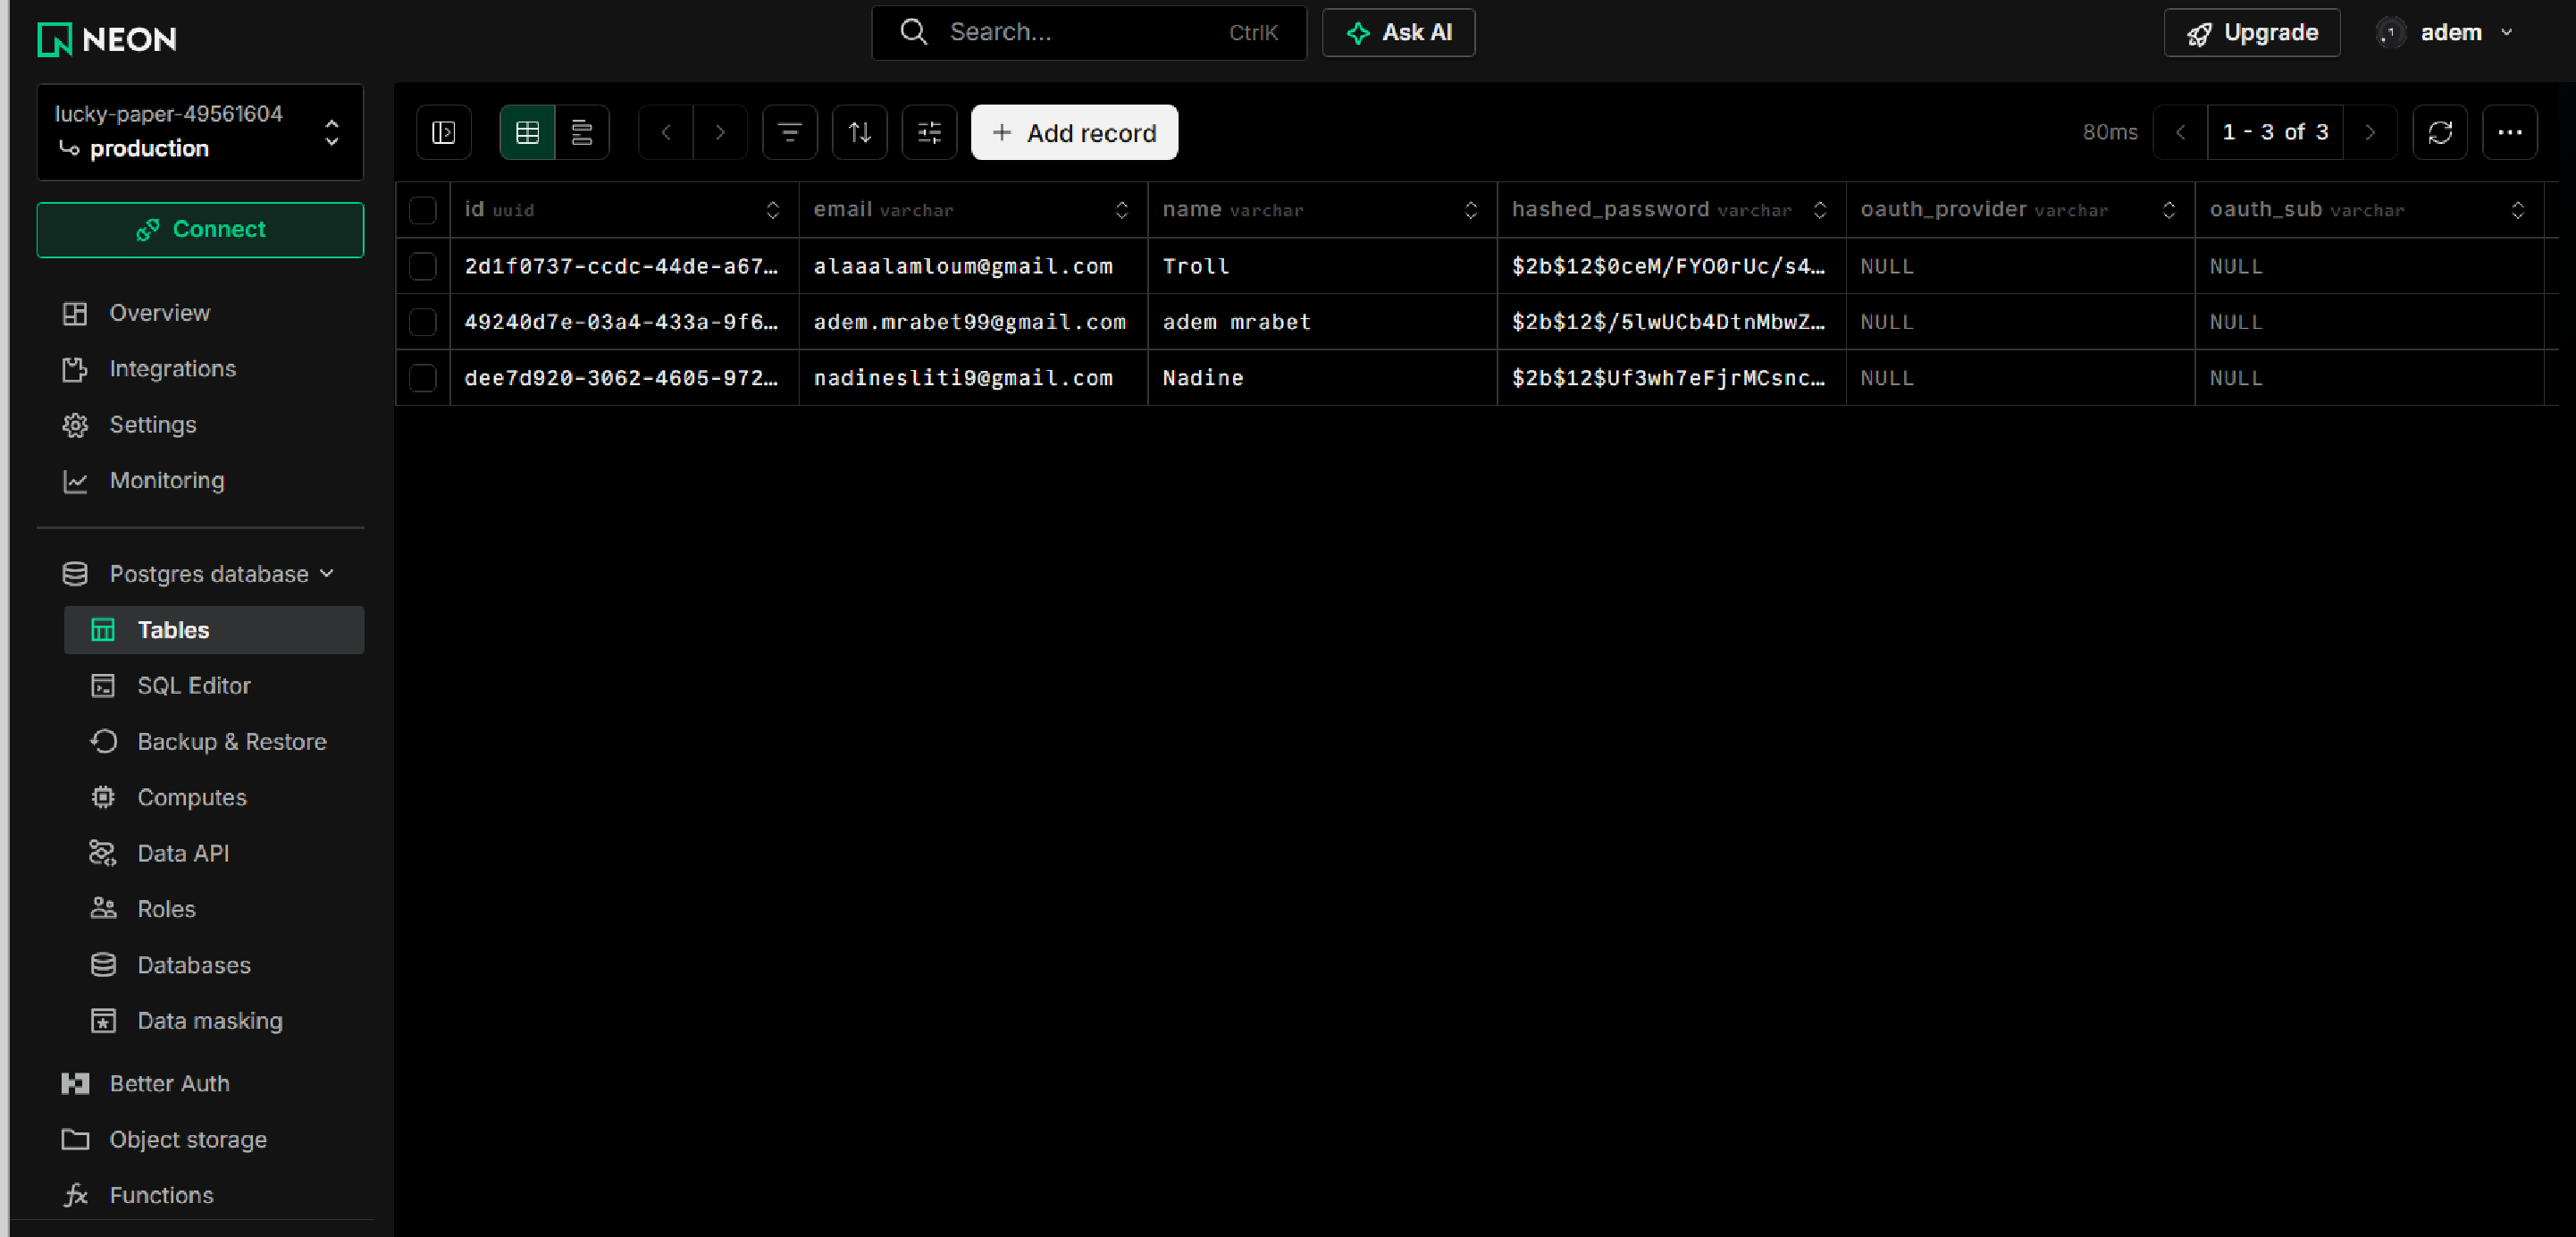
\includegraphics[width=0.98\textwidth]{figures/db-users.pdf}
\caption{Accounts table in the deployed instance. Each account carries a bcrypt
digest beginning \texttt{\$2b\$12\$}, and the federated identity columns are null for
accounts registered with a password.}
\label{fig:dbusers}
\end{figure}

\subsection{Conversations Table}

A conversation is stored as one row carrying its entire message sequence in a single JSON
column, rather than as a parent row with one child row per message. This is a deliberate
denormalisation and it deserves the scrutiny it usually attracts.

The normalised design is the textbook answer and would be correct if messages were ever
addressed individually. They are not. Every read in this application fetches a whole
conversation to display it, and every write appends to the end of one. There is no query
anywhere in the system that asks for a single message, no pagination within a conversation,
and no aggregate computed across messages. A child table would therefore contribute a join
on every read and an ordering column to maintain, in exchange for a capability nothing uses.

The second reason is that the provenance metadata attached to each answer, the resolved
identifier, the resolution method, the confidence score, the model that phrased it and the
language it was answered in, is a nested structure whose shape changed repeatedly during
development. In a column-per-field design each of those changes is a schema migration. In a
JSON column the client and the agent agree on the shape and the database stores what it is
given. Given that this metadata is only ever read back and rendered, never filtered or
joined on, the flexibility was worth more than the constraint.

The honest counterpart is stated plainly: this choice forecloses future queries such as
``how many answers fell back to the template'' without either a scan over the JSON documents
or a migration to a normalised form. That is an acceptable trade only because no such query
exists today, and it would need revisiting if the usage analytics discussed in
Section~\ref{sec:govkpi} were implemented.

Table~\ref{tab:convschema} gives the definition, and Figure~\ref{fig:dbconversations} shows
it populated.

\begin{figure}[htbp]
\centering
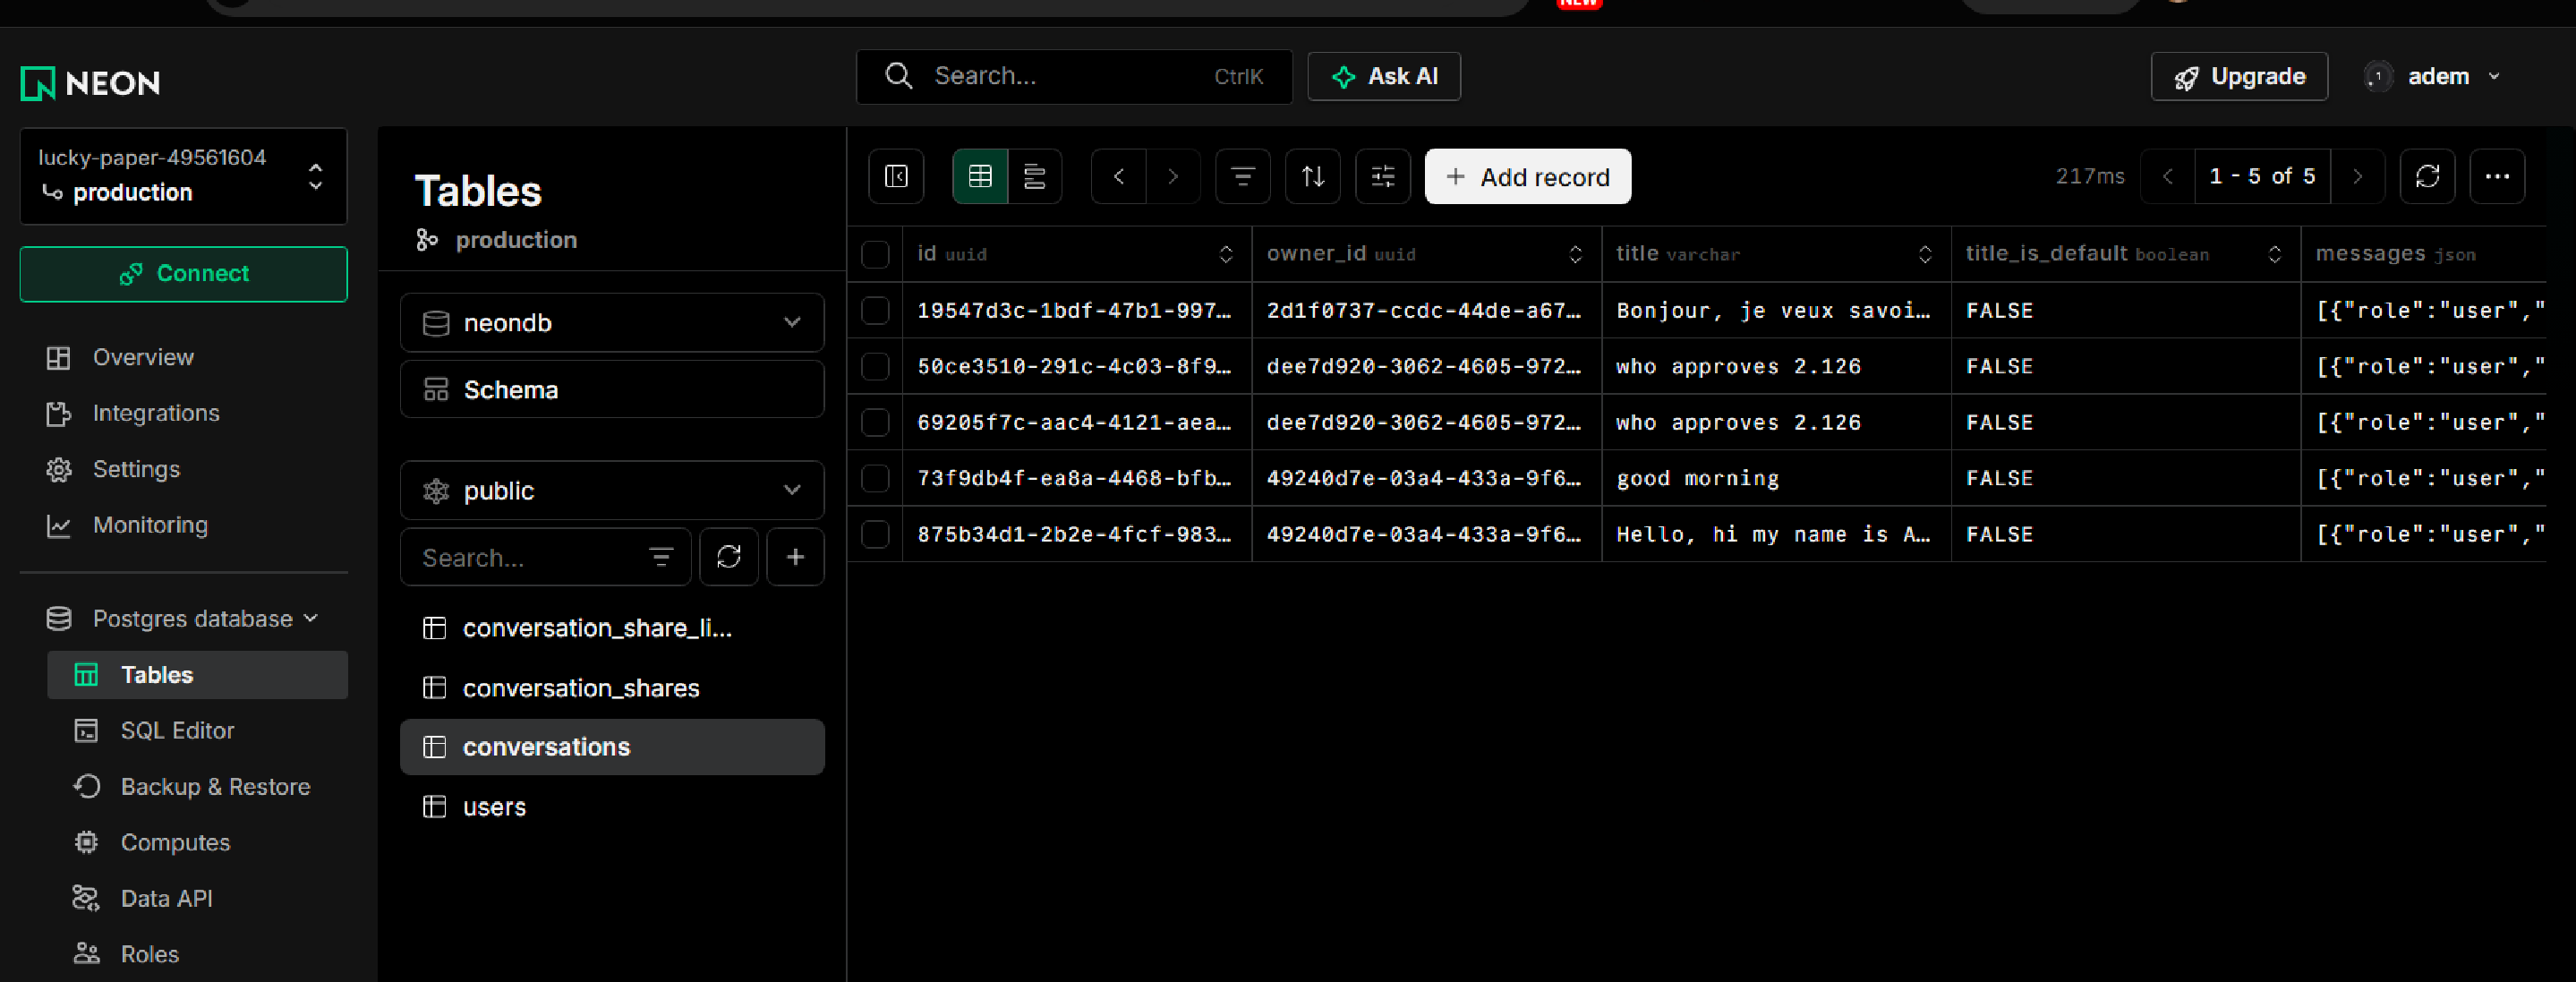
\includegraphics[width=0.98\textwidth]{figures/db-conversations.pdf}
\caption{Conversations table in the deployed instance. Each row carries a whole
thread: the owning account, the title derived from the first question, and the JSON message
column holding every exchange with its provenance metadata.}
\label{fig:dbconversations}
\end{figure}

\begin{longtable}{|p{0.22\textwidth}|p{0.16\textwidth}|p{0.52\textwidth}|}
\caption{Conversations table \texttt{conversations}.}\label{tab:convschema}\\
\hline
\rowcolor{myblue}\textcolor{white}{\textbf{Column}} & \textcolor{white}{\textbf{Type}} & \textcolor{white}{\textbf{Purpose and constraints}} \\
\hline
\endfirsthead
\hline
\rowcolor{myblue}\textcolor{white}{\textbf{Column}} & \textcolor{white}{\textbf{Type}} & \textcolor{white}{\textbf{Purpose and constraints}} \\
\hline
\endhead
\texttt{id} & UUID & Primary key. Appears in share URLs, hence random rather than sequential. \\ \hline
\texttt{owner\_id} & UUID & Foreign key to \texttt{users}, indexed. The account that created the conversation and the only one that may extend it. \\ \hline
\texttt{title} & string & Display title, defaulting to ``New chat''. \\ \hline
\texttt{title\_is\_default} & boolean & Whether the title is still the placeholder. \\ \hline
\texttt{messages} & JSON & The ordered message list, each entry carrying role, text, and provenance metadata. \\ \hline
\texttt{created\_at} & timestamp & Creation time, UTC. \\ \hline
\texttt{updated\_at} & timestamp & Maintained automatically on every write; drives sidebar ordering. \\ \hline
\end{longtable}

The \texttt{title\_is\_default} flag solves a small problem neatly enough to be worth a
sentence. A conversation should take its title from the first question asked, so that the
sidebar is navigable, but a user who renames a conversation must not have that title
overwritten by the next message. Storing the title alone cannot distinguish a placeholder
from a deliberate choice that happens to resemble one. The boolean records intent rather
than inferring it: the first message replaces the title only while the flag is set, and any
explicit rename clears it permanently.

\subsection{Sharing Tables}

Sharing is carried by two tables that do different jobs, and separating them is what keeps
authorisation coherent.

\texttt{conversation\_shares} records grants that already exist: one row per pair of
conversation and recipient. It is the single authority on who may view a conversation,
and every read path consults it. The pair is constrained unique, which makes re-sharing with
the same colleague idempotent rather than an error or a duplicate row. Two separate foreign
keys point at \texttt{users}, one for the recipient and one for the grantor, so the table
also records who extended the access rather than only that it exists.

\texttt{conversation\_share\_links} records an invitation that has not yet been accepted: a
random token, the conversation it refers to, who issued it, and when it expires, defaulting
to seven days. Crucially, a link is not itself a grant. Claiming one creates an ordinary
row in \texttt{conversation\_shares}, which means the QR-code path and the by-name path
converge on the same authorisation record, and the question of who may view a conversation
continues to have exactly one answer in the code. Had the link been treated as a credential
in its own right, every read path would have needed to check two conditions instead of one,
and the two would have drifted.

One active link is maintained per conversation. A second request for a QR code returns the
existing token rather than minting a new one, so a code already printed or already scanned
does not quietly stop working.

Table~\ref{tab:shareschema} gives both definitions, and Figure~\ref{fig:dbshares} shows a
live grant.

\begin{longtable}{|p{0.17\textwidth}|p{0.26\textwidth}|p{0.47\textwidth}|}
\caption{Two sharing tables.}\label{tab:shareschema}\\
\hline
\rowcolor{myblue}\textcolor{white}{\textbf{Table}} & \textcolor{white}{\textbf{Column}} & \textcolor{white}{\textbf{Purpose and constraints}} \\
\hline
\endfirsthead
\hline
\rowcolor{myblue}\textcolor{white}{\textbf{Table}} & \textcolor{white}{\textbf{Column}} & \textcolor{white}{\textbf{Purpose and constraints}} \\
\hline
\endhead
\texttt{conversation\_shares} & \texttt{id} & Primary key. \\ \hline
 & \texttt{conversation\_id} & Foreign key, indexed. \\ \hline
 & \texttt{shared\_with\_user\_id} & Foreign key, indexed. The account granted read access. \\ \hline
 & \texttt{shared\_by\_user\_id} & Foreign key. The account that granted it. \\ \hline
 & \texttt{created\_at} & When access was granted. \\ \hline
 & \multicolumn{2}{p{0.73\textwidth}|}{\textbf{Constraint} \texttt{uq\_conversation\_share}: (conversation, recipient) unique, making a repeat share idempotent.} \\ \hline
\texttt{conversation\_share\_links} & \texttt{id} & Primary key. \\ \hline
 & \texttt{conversation\_id} & Foreign key, indexed. \\ \hline
 & \texttt{token} & Unique and indexed. The random secret encoded into the QR image. \\ \hline
 & \texttt{created\_by\_user\_id} & Foreign key. Who issued the link. \\ \hline
 & \texttt{created\_at} & Issue time. \\ \hline
 & \texttt{expires\_at} & Expiry, defaulting to seven days after issue. \\ \hline
\end{longtable}

\begin{figure}[htbp]
\centering
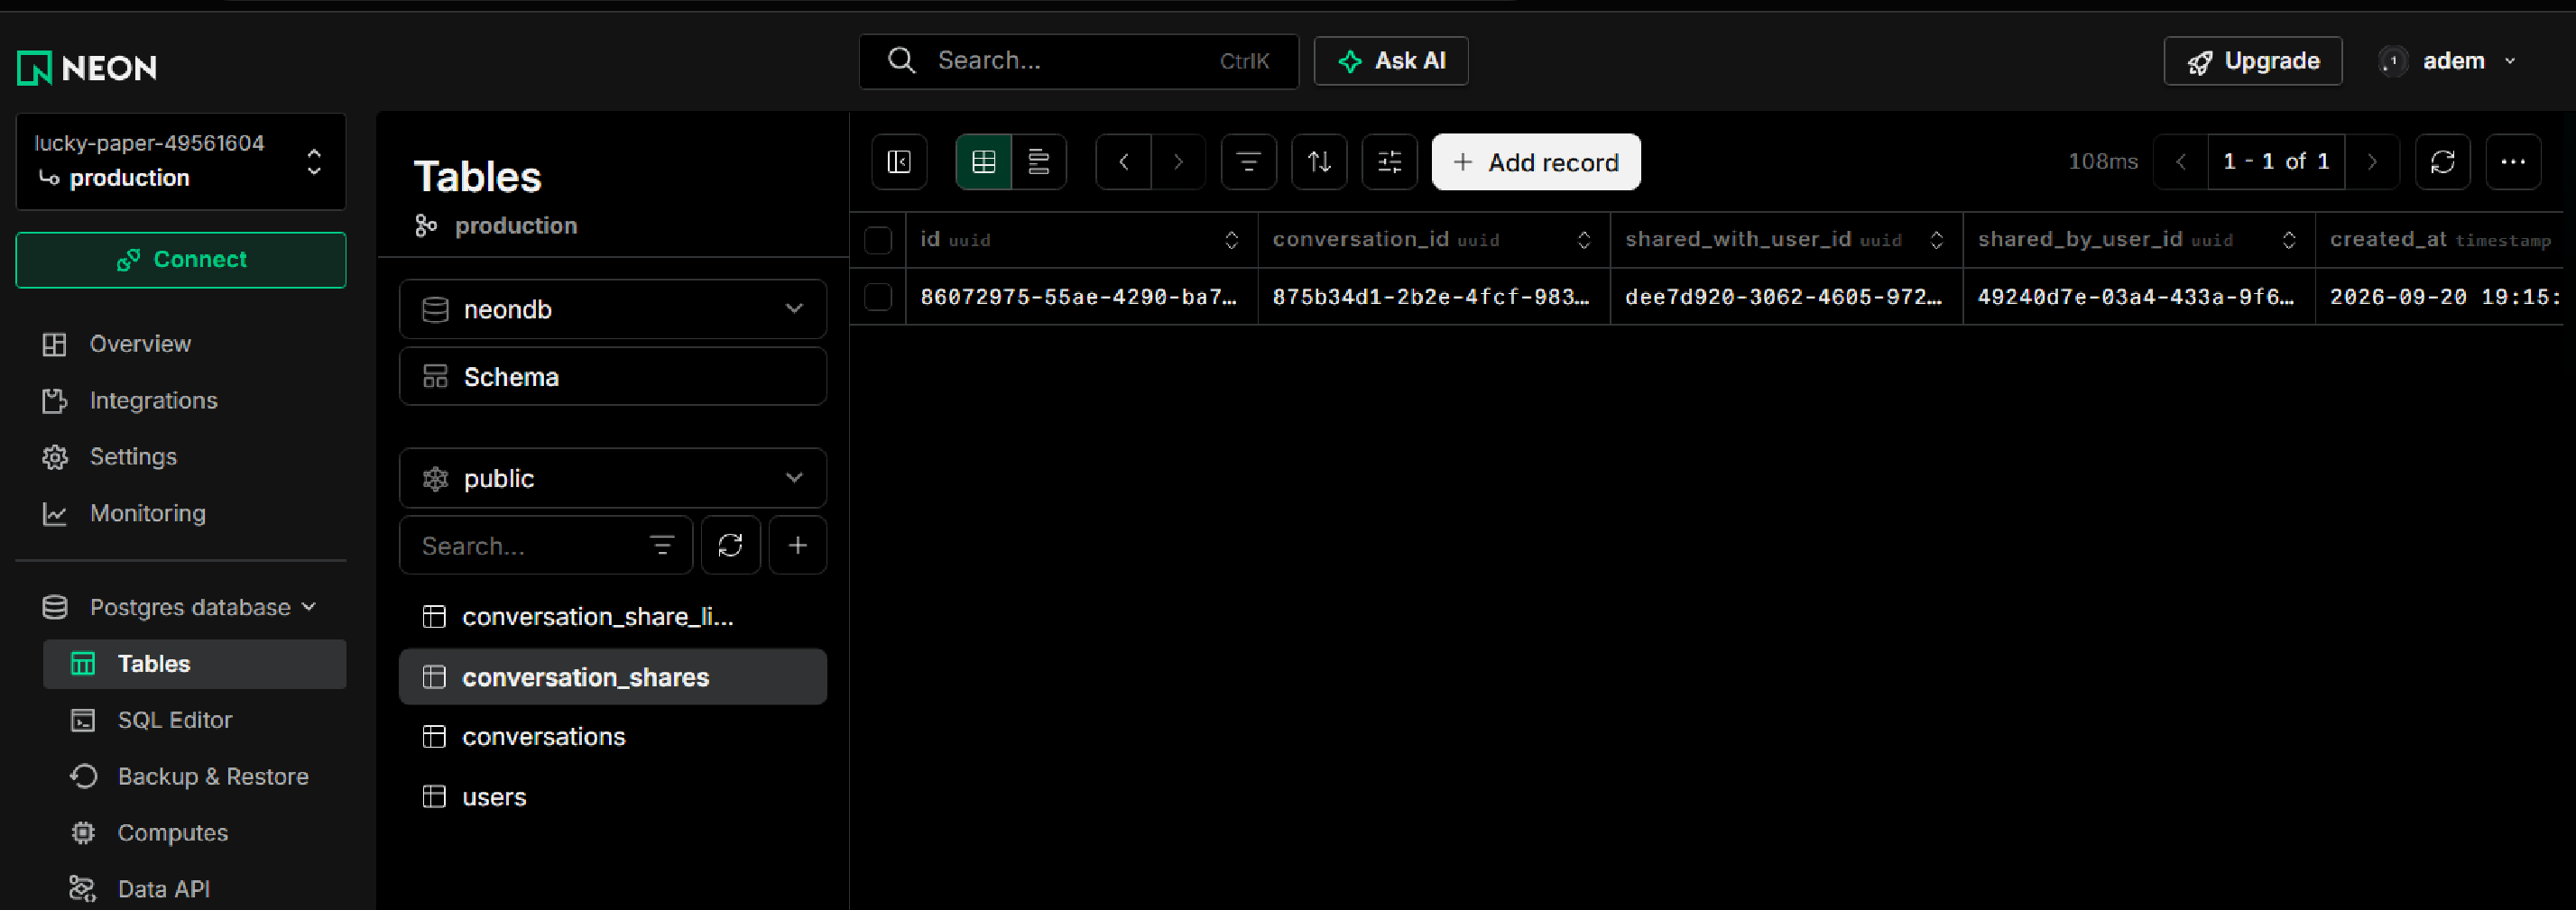
\includegraphics[width=0.98\textwidth]{figures/db-shares.pdf}
\caption{Sharing grants held in \texttt{conversation\_shares}, showing one live grant. The row names the
conversation, the account granted access, and the account that granted it.}
\label{fig:dbshares}
\end{figure}

\subsection{Referential Integrity and Deletion}

Both sharing tables are declared as dependants of the conversation with delete-orphan
cascade, so removing a conversation removes its grants and its outstanding links in the same
operation. This matters more than ordinary tidiness. Without the cascade, deleting a
conversation would leave grant rows pointing at an identifier that no longer resolves, and an
outstanding share link would remain valid in the sense that its token still existed and had
not expired. Access-control records that outlive the thing they protect are precisely the
kind of residue that later produces a security incident, so the lifetime of a grant is bound
to the lifetime of its conversation at the schema level rather than in application code that
might be bypassed.

One implementation detail is worth recording because it caused a real error. The share table
holds two foreign keys into \texttt{users}, and the mapper cannot infer which one a given
relationship traverses when more than one candidate exists; both relationships therefore
declare their join column explicitly. The error surfaces at mapper configuration time rather
than at query time, which is the preferable failure, but it is opaque enough on first
encounter to be worth naming here.

\section{Access Control}

Ownership is the concept this whole section serves: nothing about persistence or sharing
means anything until the system can say whose conversation it is looking at.
Figure~\ref{fig:applogin} shows the sign-in screen the decisions below sit behind.

\begin{figure}[htbp]
\centering
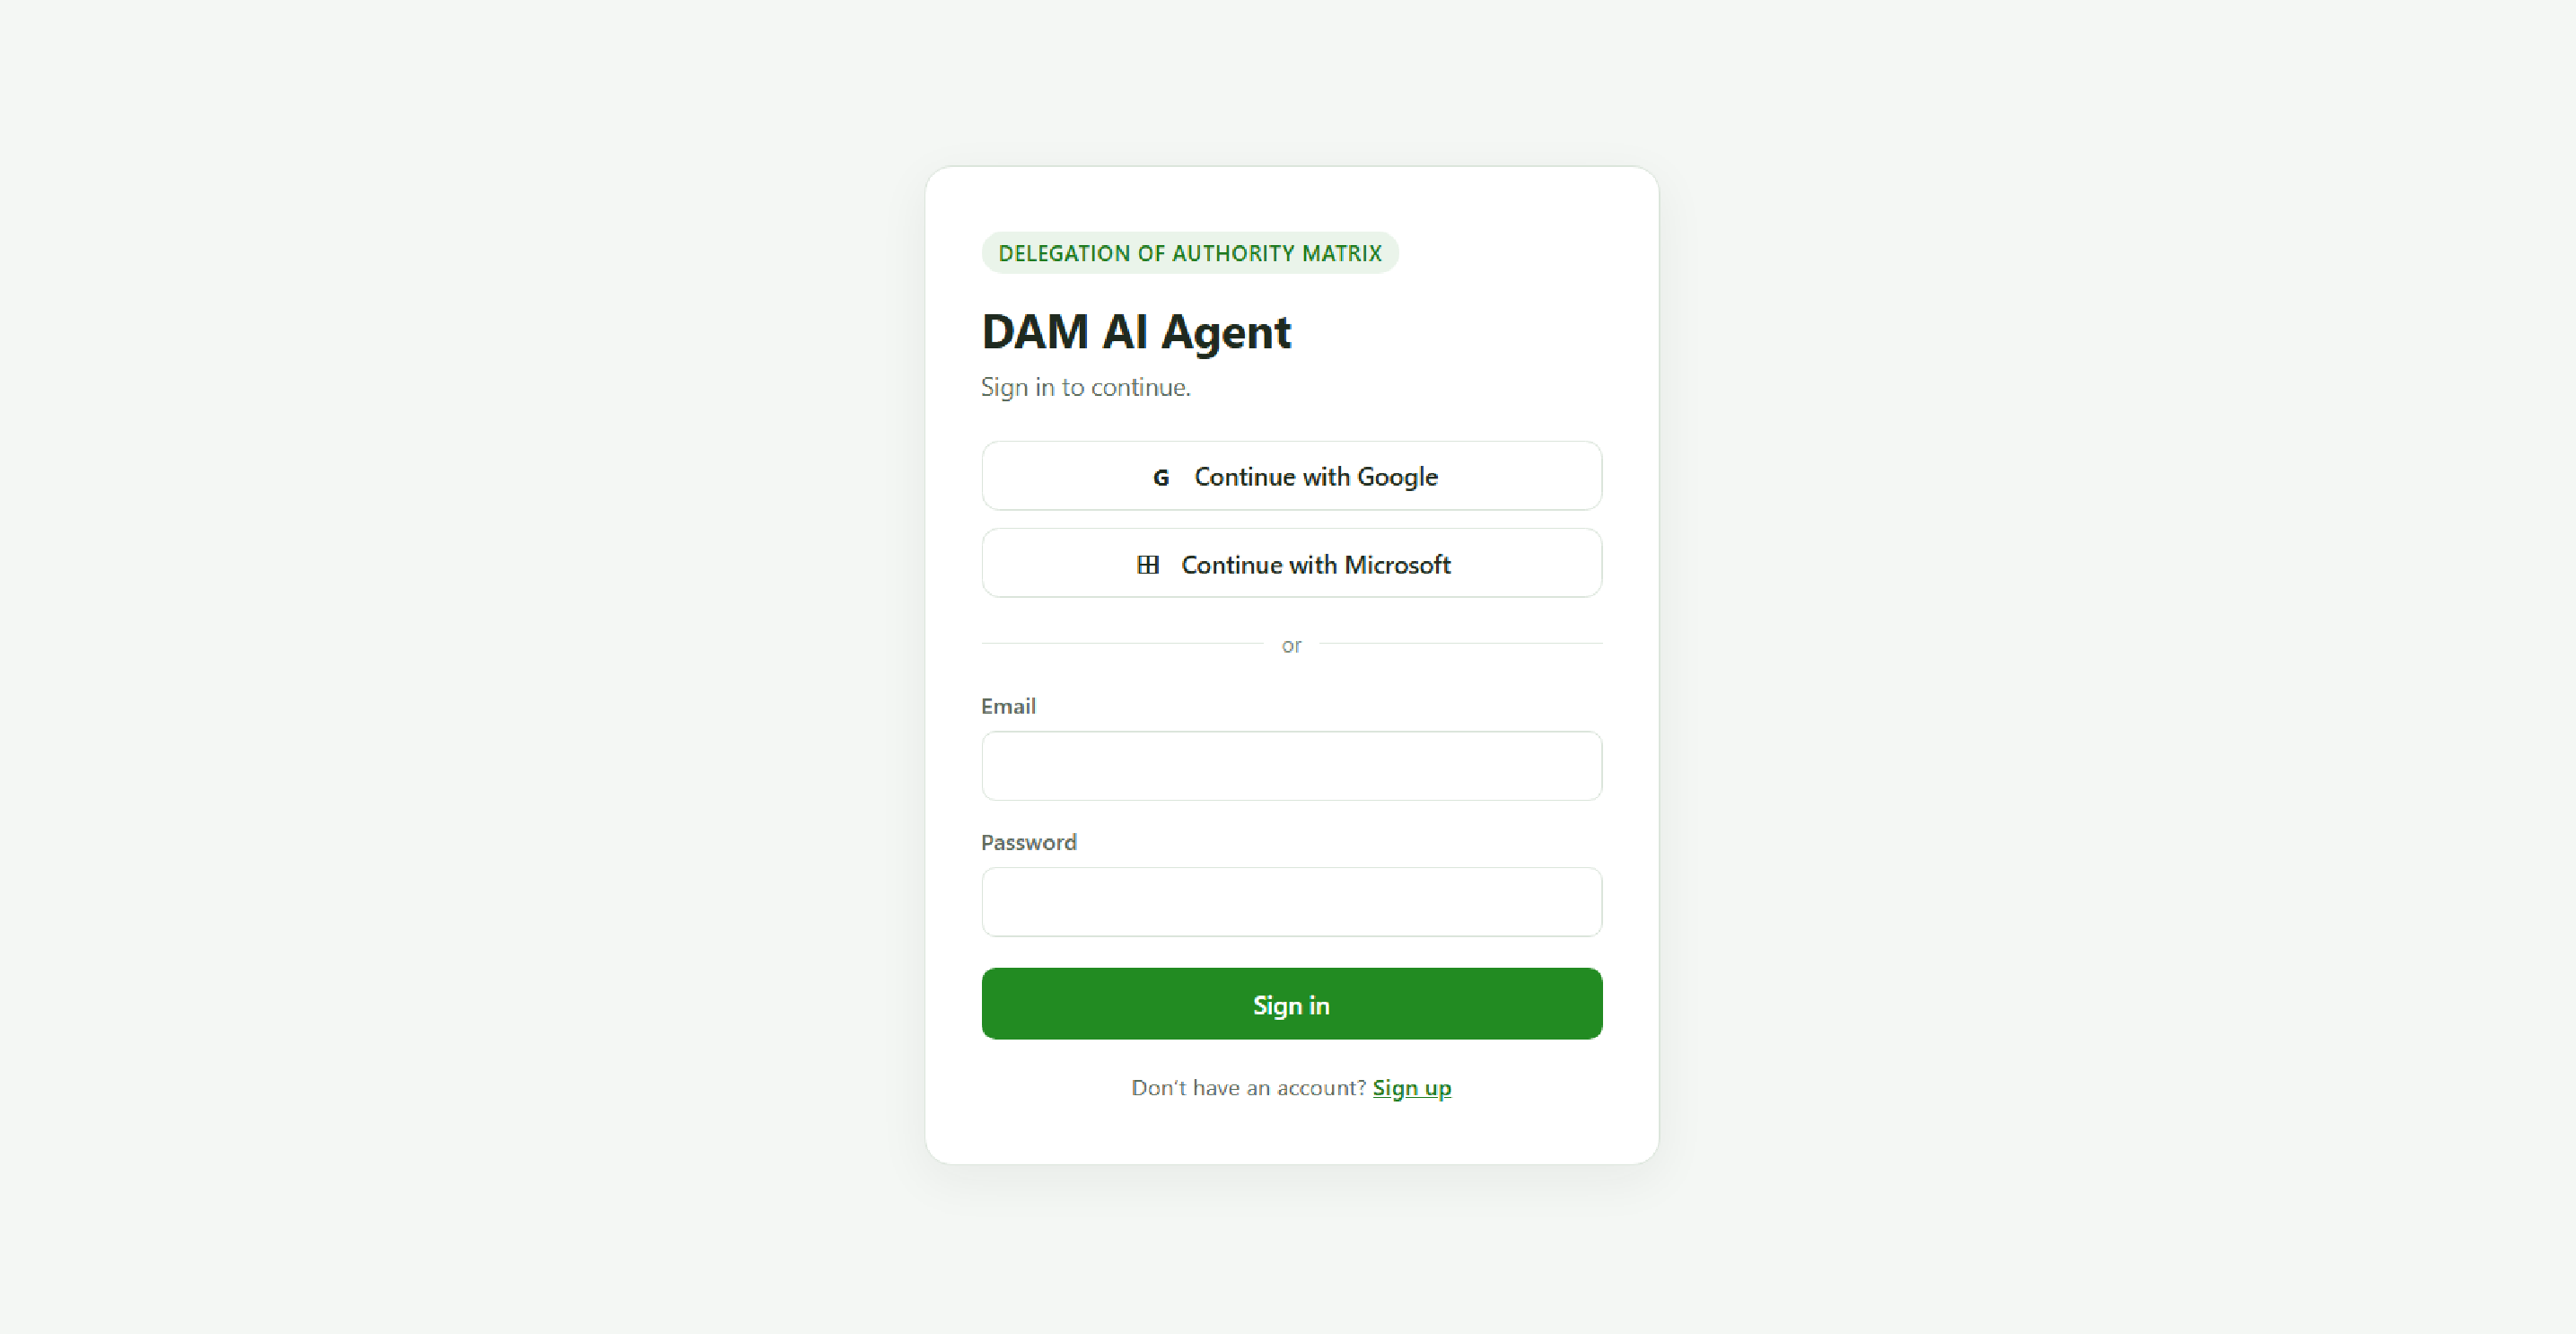
\includegraphics[width=0.55\textwidth]{figures/app-login.pdf}
\caption{Sign-in screen, offering federated sign-in through Google or Microsoft alongside
the email-and-password form.}
\label{fig:applogin}
\end{figure}

\subsection{Why Authentication Was Necessary}

The first version of this system had no accounts. Anyone reaching the service could ask
questions, and conversations lived in the browser's own storage. That was adequate while the
system did one thing, and it stopped being adequate the moment conversations needed to be
persisted and shared, for a reason that is structural rather than incidental: sharing
requires ownership, ownership requires identity, and identity requires authentication. There
is no way to grant a colleague access to something that belongs to nobody.

A second reason is specific to this subject matter. The analytics layer aggregates the
delegation structure of the institution, which is organisationally sensitive in a way that a
single lookup is not, and restricting it requires being able to tell who is asking.

\subsection{Password Storage}

Passwords are never stored in a form from which the original can be recovered. Each account
holds a bcrypt digest, produced through the passlib library, and verification re-derives a
digest from the submitted password and compares the two. Bcrypt was chosen over a
general-purpose cryptographic hash for reasons worth setting out, since the distinction is
frequently elided.

A hash such as SHA-256 is designed to be fast, which is the correct property for verifying
file integrity and precisely the wrong one for storing passwords: speed is exactly what an
attacker holding a stolen database wants, since it lets them test billions of candidate
passwords per second on commodity hardware. Bcrypt is deliberately slow and, more
importantly, adjustably slow. Its cost parameter sets the number of key-expansion rounds as a
power of two, and raising it by one doubles the work required both for a legitimate
verification and for every guess an attacker makes. The digests in this system carry a cost
of twelve, meaning $2^{12}$ rounds, which is visible in the \texttt{\$2b\$12\$} prefix of
every stored value in Figure~\ref{fig:dbusers}. The parameter is stored alongside the digest
rather than fixed in code, so the cost can be raised as hardware improves and existing
accounts continue to verify against their original setting until their next successful login.

Bcrypt also salts each password individually and stores the salt in the same field. The
consequence is that two accounts choosing the same password hold entirely different digests,
which defeats both precomputed rainbow tables and the simpler attack of noticing that two
rows share a value and therefore share a password.

The interaction between password storage and federated accounts is the property described
earlier: an account authenticated through a provider carries no digest at all, and the login
endpoint refuses it before any comparison is attempted.

\subsection{Token Design}

Authentication is stateless. A successful sign-in returns a signed JSON Web
Token\citep{rfc7519}, and the client presents it in the \texttt{Authorization} header of
every subsequent request. Table~\ref{tab:jwtclaims} lists what the token asserts.

\begin{longtable}{|p{0.14\textwidth}|p{0.30\textwidth}|p{0.46\textwidth}|}
\caption{Claims carried by the access token.}\label{tab:jwtclaims}\\
\hline
\rowcolor{myblue}\textcolor{white}{\textbf{Claim}} & \textcolor{white}{\textbf{Value}} & \textcolor{white}{\textbf{Why it is present}} \\
\hline
\endfirsthead
\hline
\rowcolor{myblue}\textcolor{white}{\textbf{Claim}} & \textcolor{white}{\textbf{Value}} & \textcolor{white}{\textbf{Why it is present}} \\
\hline
\endhead
\texttt{sub} & Account UUID & Identifies the caller. Every ownership check resolves from this. \\ \hline
\texttt{email} & Address & Lets the interface show the signed-in account without an extra request. \\ \hline
\texttt{role} & \texttt{analyst} or \texttt{administrator} & Carries the authorisation decision, avoiding a lookup on every request. \\ \hline
\texttt{iat} & Issue time & Establishes token age. \\ \hline
\texttt{exp} & Issue time plus eight hours & Bounds the damage a leaked token can do. \\ \hline
\end{longtable}

The token is signed HS256\citep{rfc7515}, a keyed signature using a secret held only by the
server. Signing establishes integrity, not confidentiality: the claims are encoded, not
encrypted, and anyone holding the token can read them. Nothing secret is therefore placed in
it. What signing guarantees is that a client cannot alter a claim, and the claim that matters
is \texttt{role}: without a signature, elevating oneself to administrator would be a matter
of editing a string.

The signing secret is read from the environment with no fallback default, so a deployment
that has not configured one fails immediately at startup rather than silently signing tokens
with a value an attacker could guess from the source. Failing loudly at boot is the correct
behaviour for a misconfiguration of this class.

Expiry is eight hours, chosen to span a working day. The trade-off is explicit: a shorter
window would force repeated sign-ins during ordinary use, and a longer one would leave a
usable credential in a browser long after the person had finished. Because verification is
stateless, a token cannot be revoked before it expires, which is the cost of not consulting
the database on every request. For this application that cost is acceptable; a system holding
higher-value operations would need a revocation list and the lookup that comes with it.

On the client the token is held in session storage rather than local storage. Both are
readable by any script executing on the page, so the distinction is not about resisting
script access; it is about lifetime. Session storage is cleared when the tab closes, whereas
local storage persists indefinitely, leaving a valid credential on a shared or unattended
machine long after the user believed they had finished. The cost is that closing the tab
requires signing in again, which was judged the right trade for a system holding governance
information.

\subsection{Federated Sign-In}

Two federated paths exist alongside the password form, through Google and through Microsoft.
The motivation is institutional rather than technical: staff at an organisation of this kind
already hold a corporate directory account, and requiring a separate password adds a
credential to be managed, forgotten, reused, or written down, while removing the ability of
the institution to revoke access centrally when someone leaves.

Both providers are integrated through OpenID Connect rather than by hand-coded calls to
provider endpoints. The client is configured with a discovery document URL, and the endpoints,
signing keys and supported parameters are retrieved from the provider at runtime. This matters
for durability: a provider rotating its signing keys or relocating an endpoint does not break
the integration, because nothing about those details is hardcoded. The requested scope is the
minimum the application needs, namely the identity token plus the address and display name.
The Microsoft integration additionally accepts a tenant identifier, defaulting to the
multi-tenant endpoint, so that the same build can be pointed at a single institutional
directory by configuration alone.

Both providers are registered only when their credentials are present in the environment. An
instance configured with neither still starts and still serves password sign-in, which keeps
local development and the test suite free of any dependency on external identity services.

\subsection{Resolving a Federated Identity to an Account}

The step where a provider's response becomes a local account is the most security-sensitive
part of the flow, and the order of the lookups is the substance of it.

The account is located first by the pair of provider and subject identifier, the provider's
own immutable handle for that person, and never by email address alone. This ordering is
deliberate. Email addresses are not stable identifiers: an organisation may reassign a
departed employee's address to a new hire, and a person may change their own address at the
provider. A system matching on email alone would hand the new holder of a recycled address
the previous holder's account and every conversation in it. Matching on the subject
identifier makes that impossible, because the identifier is never reissued.

Only when no account carries that provider identity does the resolution fall back to email,
and then only to link the provider identity onto an existing account rather than to
authenticate against it. This is what lets a user who registered with a password later sign
in through Google and arrive at the same account rather than a duplicate. The account is
created fresh only when both lookups fail.

The uniqueness constraint on the provider-and-subject pair enforces the invariant at the
database level, so a defect in this logic cannot produce two local accounts claiming the same
provider identity.

Figure~\ref{fig:authflow} lays out the same decision as a flowchart, since the order in
which the three checks run is the part of this logic most likely to be got wrong by a
future change.

\begin{figure}[htbp]
\centering
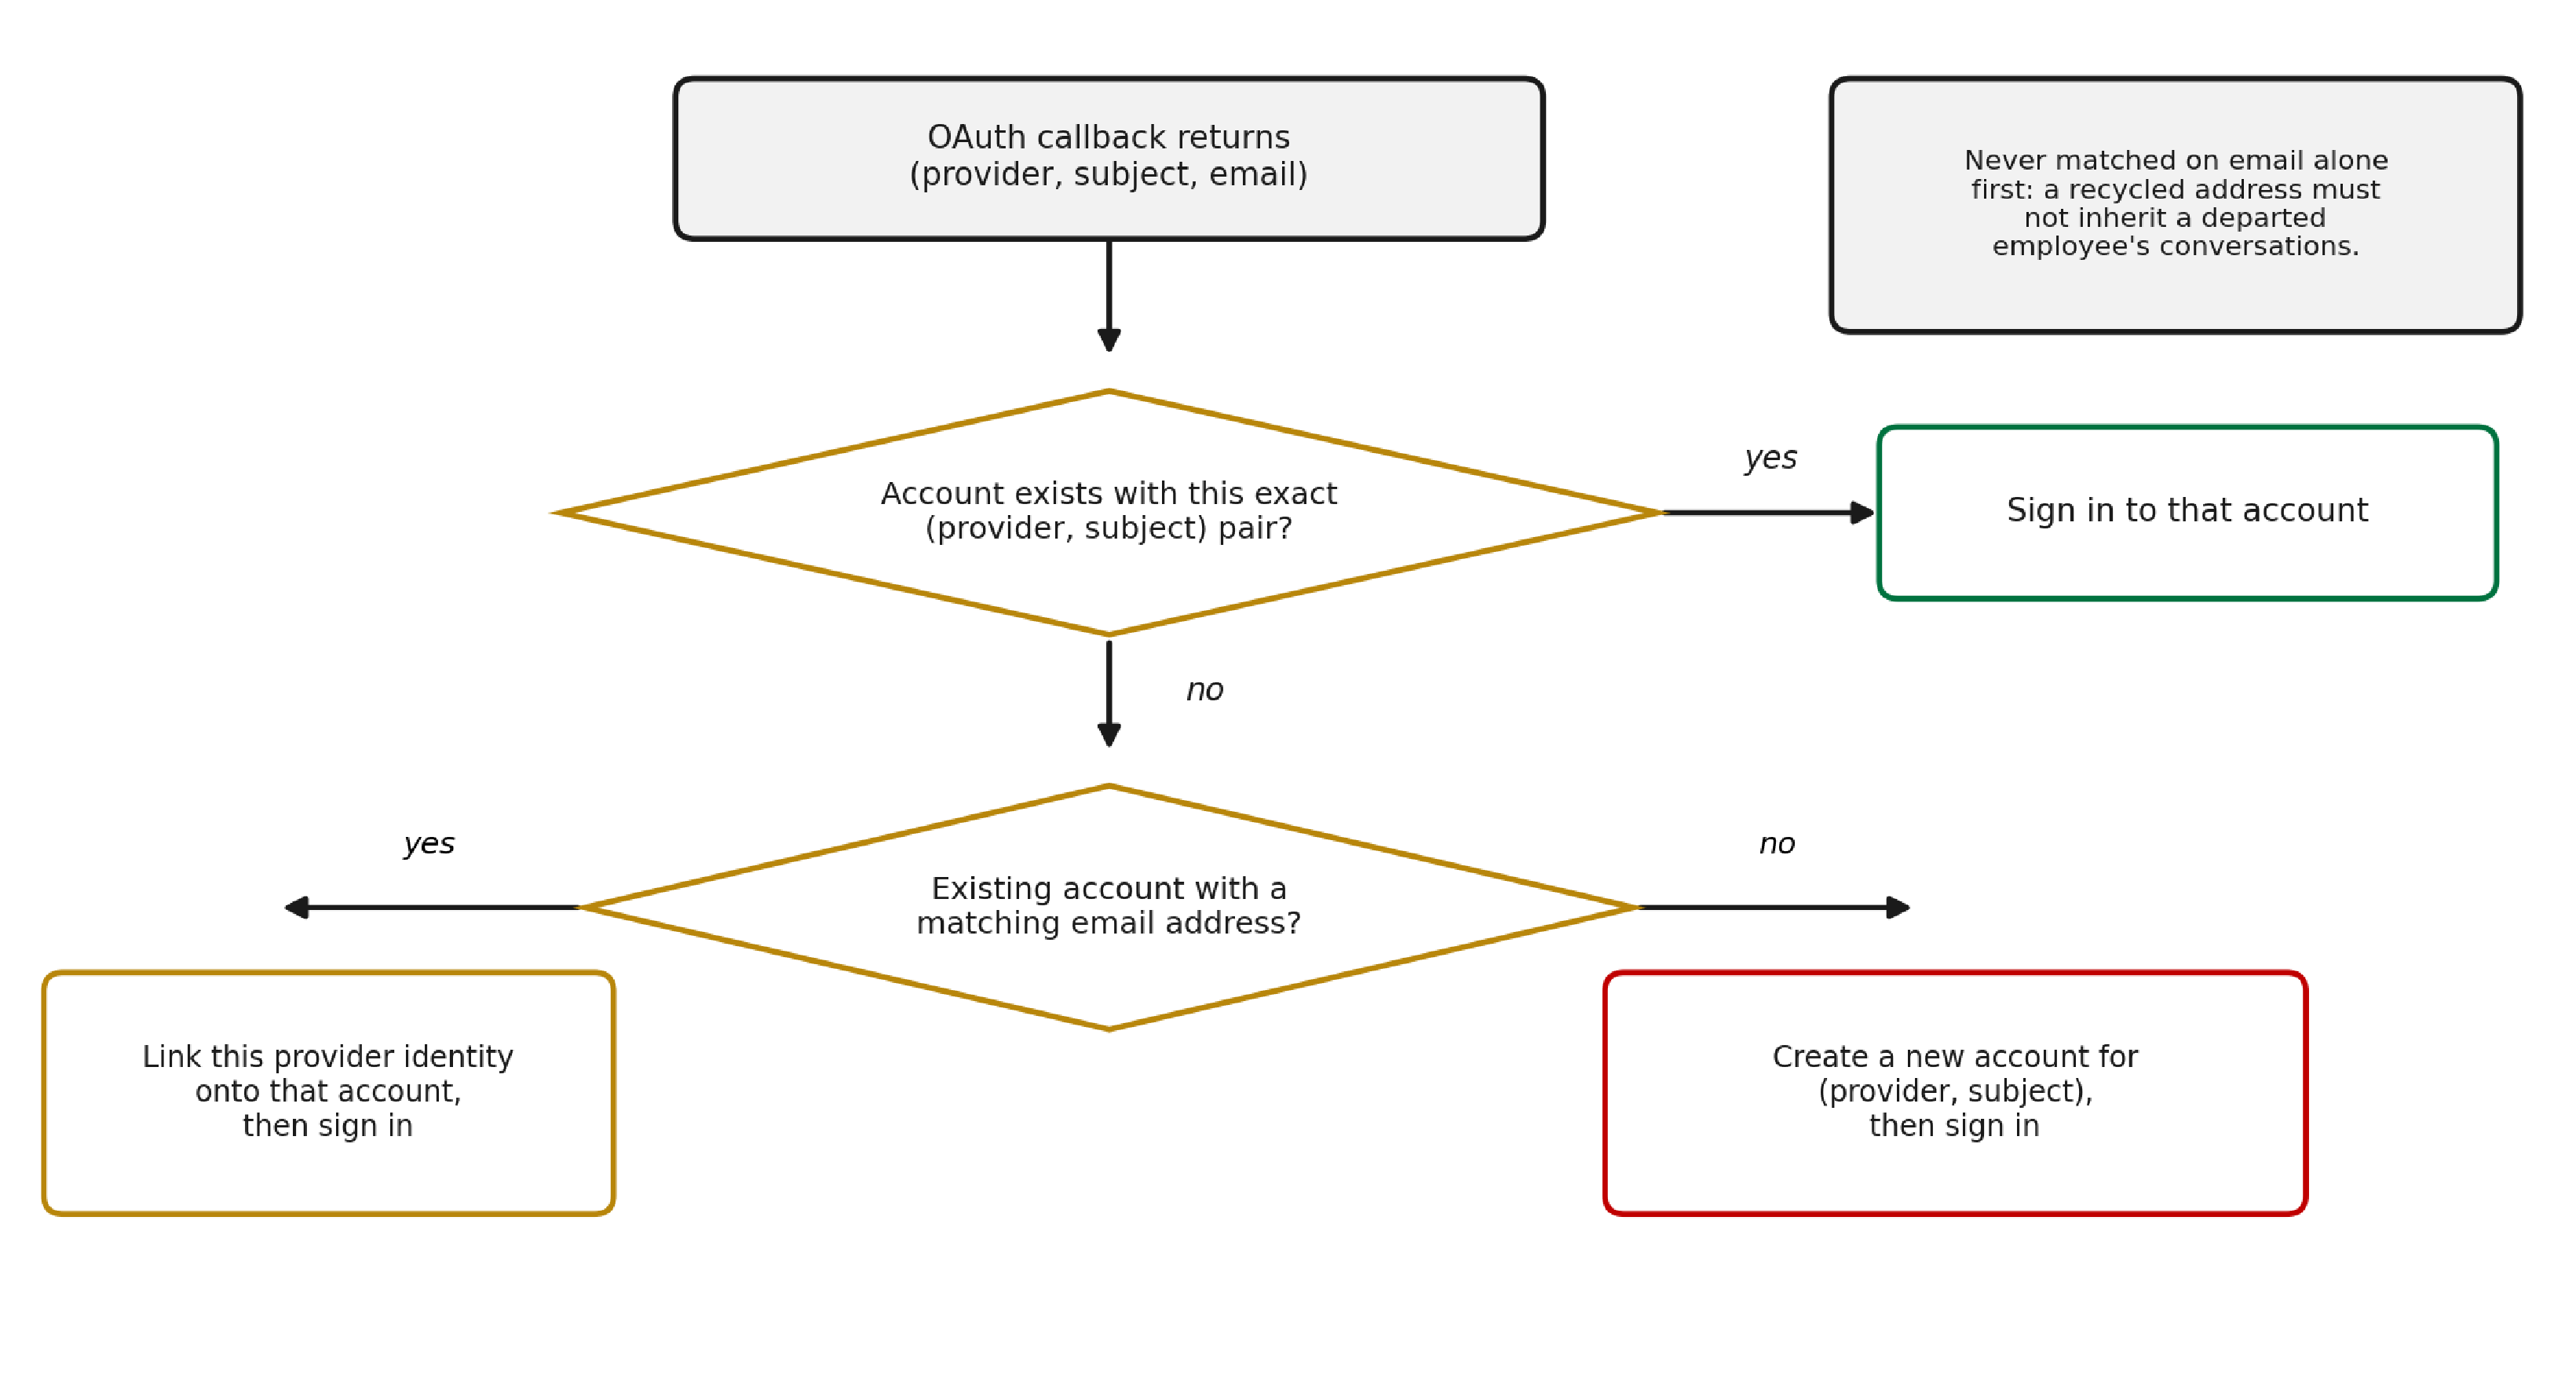
\includegraphics[width=0.92\textwidth]{figures/fig-authflow.pdf}
\caption{Resolving a federated identity to a local account. The provider-and-subject pair is
checked first and email is consulted only as a fallback for linking, never for
authentication.}
\label{fig:authflow}
\end{figure}

\subsection{Roles and Authorisation}

Two roles are defined. An \textbf{analyst} may ask questions, attach documents, and own and
share conversations. An \textbf{administrator} may additionally open the analytics dashboard.
The distinction reflects the sensitivity difference described earlier: an individual
conversation reveals what one person asked, whereas the dashboard aggregates the institution's
delegation structure.

Authorisation is enforced server-side as a dependency on the protected routes rather than by
hiding controls in the interface. An analyst who constructs the request by hand is refused
exactly as one who clicks, which is the only enforcement that means anything; a hidden button
is a usability affordance, not a control.

The first account created on an empty database becomes an administrator, which solves the
bootstrap problem of needing an administrator before one can be appointed. This is recorded as
a deliberate convenience rather than a complete design: promoting a second administrator still
requires a direct database edit, and a production deployment would want an administrative
interface for it.

\subsection{Hardening the Sign-In Path}

Three further protections apply specifically to authentication, and
Table~\ref{tab:threatmodel} sets out what each defends against.

Failed attempts are rate-limited by source address within a rolling five-minute window, which
raises the cost of credential stuffing from free to impractical without locking out a
legitimate user who has mistyped a password twice.

A failed sign-in returns one generic message regardless of whether the account exists. The
temptation to be helpful here, by saying that no account was found, produces an oracle that
converts a list of institutional email addresses into a list of confirmed users. The
implementation is careful on a related point: the same generic refusal is returned when an
account exists but has no password because it is federated, so the response does not
distinguish that case either.

A minimum password length of eight characters is enforced at registration. This is a weak
control on its own and is stated as such; it raises the floor without pretending to establish
password quality.

\begin{longtable}{|p{0.30\textwidth}|p{0.56\textwidth}|}
\caption{Authentication threats and the corresponding mitigation.}\label{tab:threatmodel}\\
\hline
\rowcolor{myblue}\textcolor{white}{\textbf{Threat}} & \textcolor{white}{\textbf{Mitigation in this system}} \\
\hline
\endfirsthead
\hline
\rowcolor{myblue}\textcolor{white}{\textbf{Threat}} & \textcolor{white}{\textbf{Mitigation in this system}} \\
\hline
\endhead
Database disclosure exposing passwords & Only salted bcrypt digests at cost twelve are stored; federated accounts hold no digest at all. \\ \hline
Offline brute-force against stolen digests & Bcrypt's cost parameter makes each guess expensive, and the parameter can be raised without a migration. \\ \hline
Rainbow-table attack & Per-password salts make precomputation useless and hide the fact that two accounts share a password. \\ \hline
Account enumeration & One generic refusal for unknown account, wrong password, and federated account alike. \\ \hline
Credential stuffing & Rate limiting per source address over a rolling window. \\ \hline
Privilege escalation by editing a token & The role claim is covered by the HS256 signature; any alteration invalidates the token. \\ \hline
Credential left on a shared machine & Tokens held in session storage, discarded when the tab closes, and expiring after eight hours regardless. \\ \hline
Conversation URL enumeration & Random UUID identifiers rather than sequential integers, with the ownership check retained as well. \\ \hline
Recycled email address inheriting an account & Federated identities resolved by immutable provider subject identifier before email is ever consulted. \\ \hline
Stale access after a conversation is deleted & Grants and outstanding links removed by database cascade with the conversation itself. \\ \hline
Misconfigured deployment signing with a default secret & The signing secret has no default; a deployment without one fails at startup. \\ \hline
\end{longtable}

\section{Conversation Interface}

With sign-in in place, what a signed-in user actually does becomes the subject: ask a
question, dictate it instead of typing, attach a document to be questioned separately from
the DAM, or read the interface in their own language. Each input mode runs through the same
underlying answer pipeline from Chapter~\ref{ch:agent}, since none of them change what an
answer is, only how the question reaches it.

\subsection{Asking a Question}

The chat page is the primary interface. A question is typed or dictated, and the answer
returns accompanied by the metadata that makes it checkable: the resolved activity
identifier, the resolution method, the confidence score where one applies, whether a
language model phrased the response, and the language the answer is written in.
Figure~\ref{fig:appchat} shows an exchange in which the agent first declines to guess at
an under-specified question and offers candidate activities, then answers the follow-up
by identifier at full confidence.

\begin{figure}[htbp]
\centering
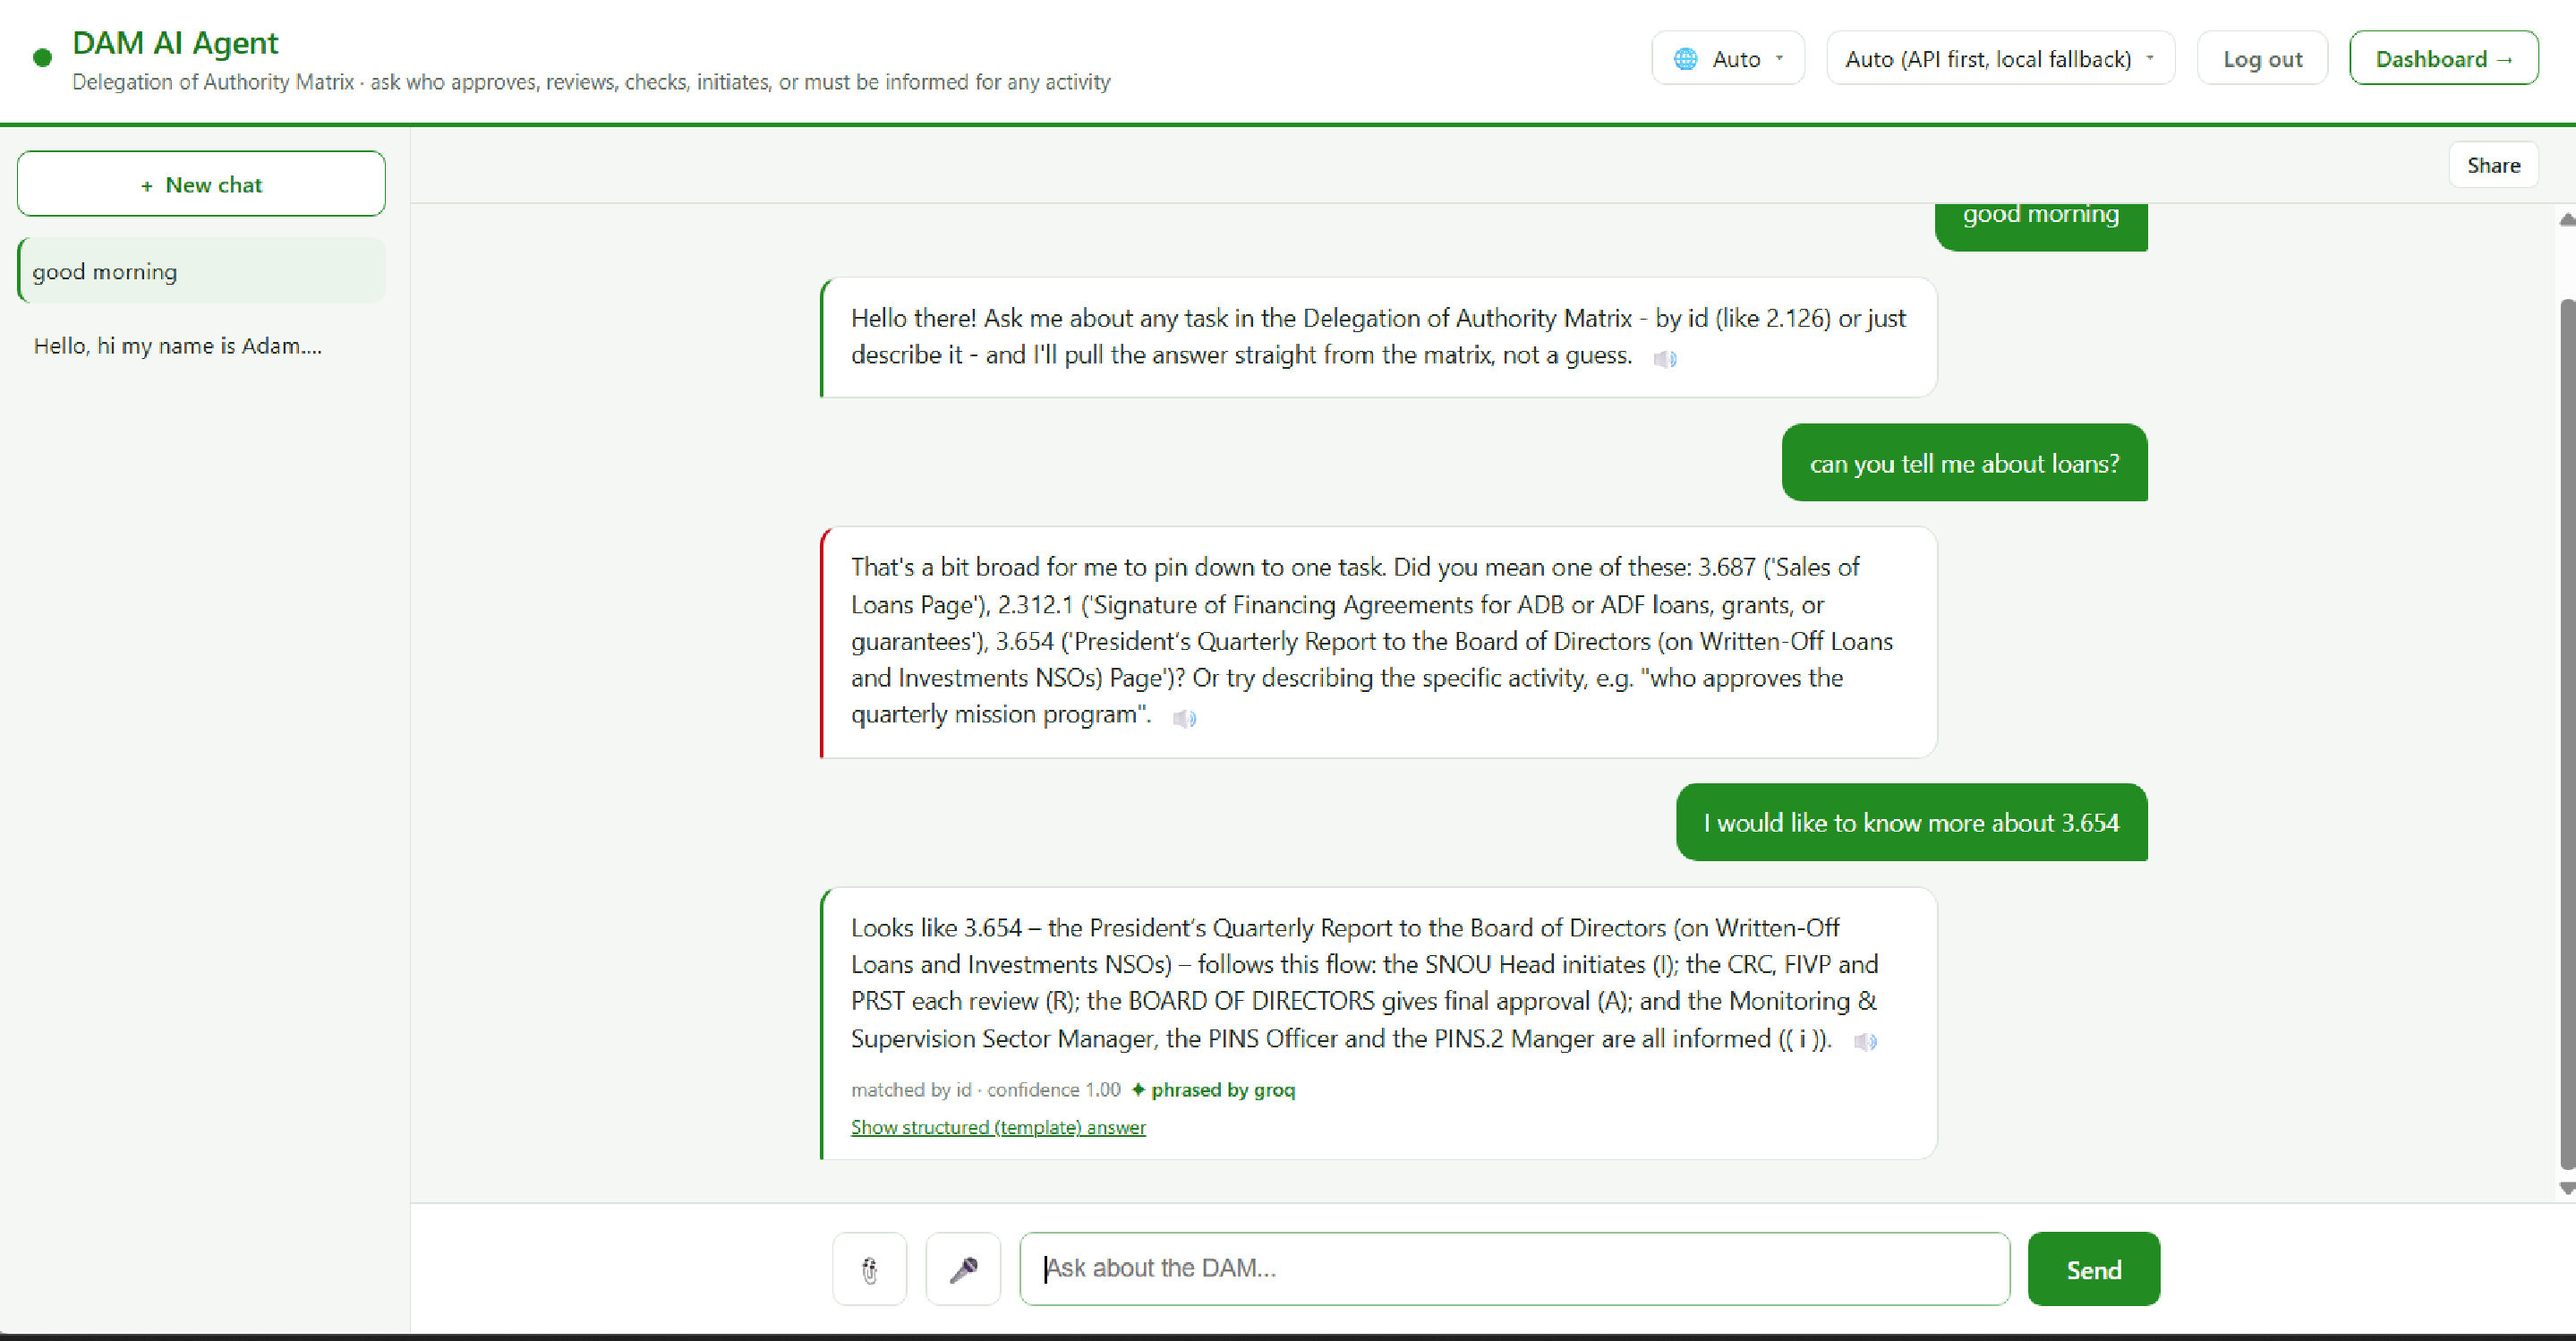
\includegraphics[width=0.95\textwidth]{figures/app-chat.pdf}
\caption{Conversation interface. The first answer refuses an under-specified question
and offers candidates rather than guessing; the second resolves by identifier at
confidence 1.0 and carries its provenance beneath the answer.}
\label{fig:appchat}
\end{figure}

Header controls select the language model mode, as set out in Table~\ref{tab:llm},
including switching it off entirely, and select the answer language. Beneath any answer a
model has phrased, a control reveals the deterministic template answer underneath it, so a
user can compare the readable sentence against the unembellished statement of what the
matrix records. This control is the interface expression of the architectural separation
argued for in Chapter~\ref{ch:agent}: the two layers remain visibly distinct at the point
of use, rather than being merged into a single authoritative-sounding paragraph.

The landing page, shown in Figure~\ref{fig:applanding}, states the same distinction before
a user has asked anything, since the difference between an answer retrieved from a
structured source and an answer generated from a document is precisely the expectation a
new user arrives with.

\begin{figure}[htbp]
\centering
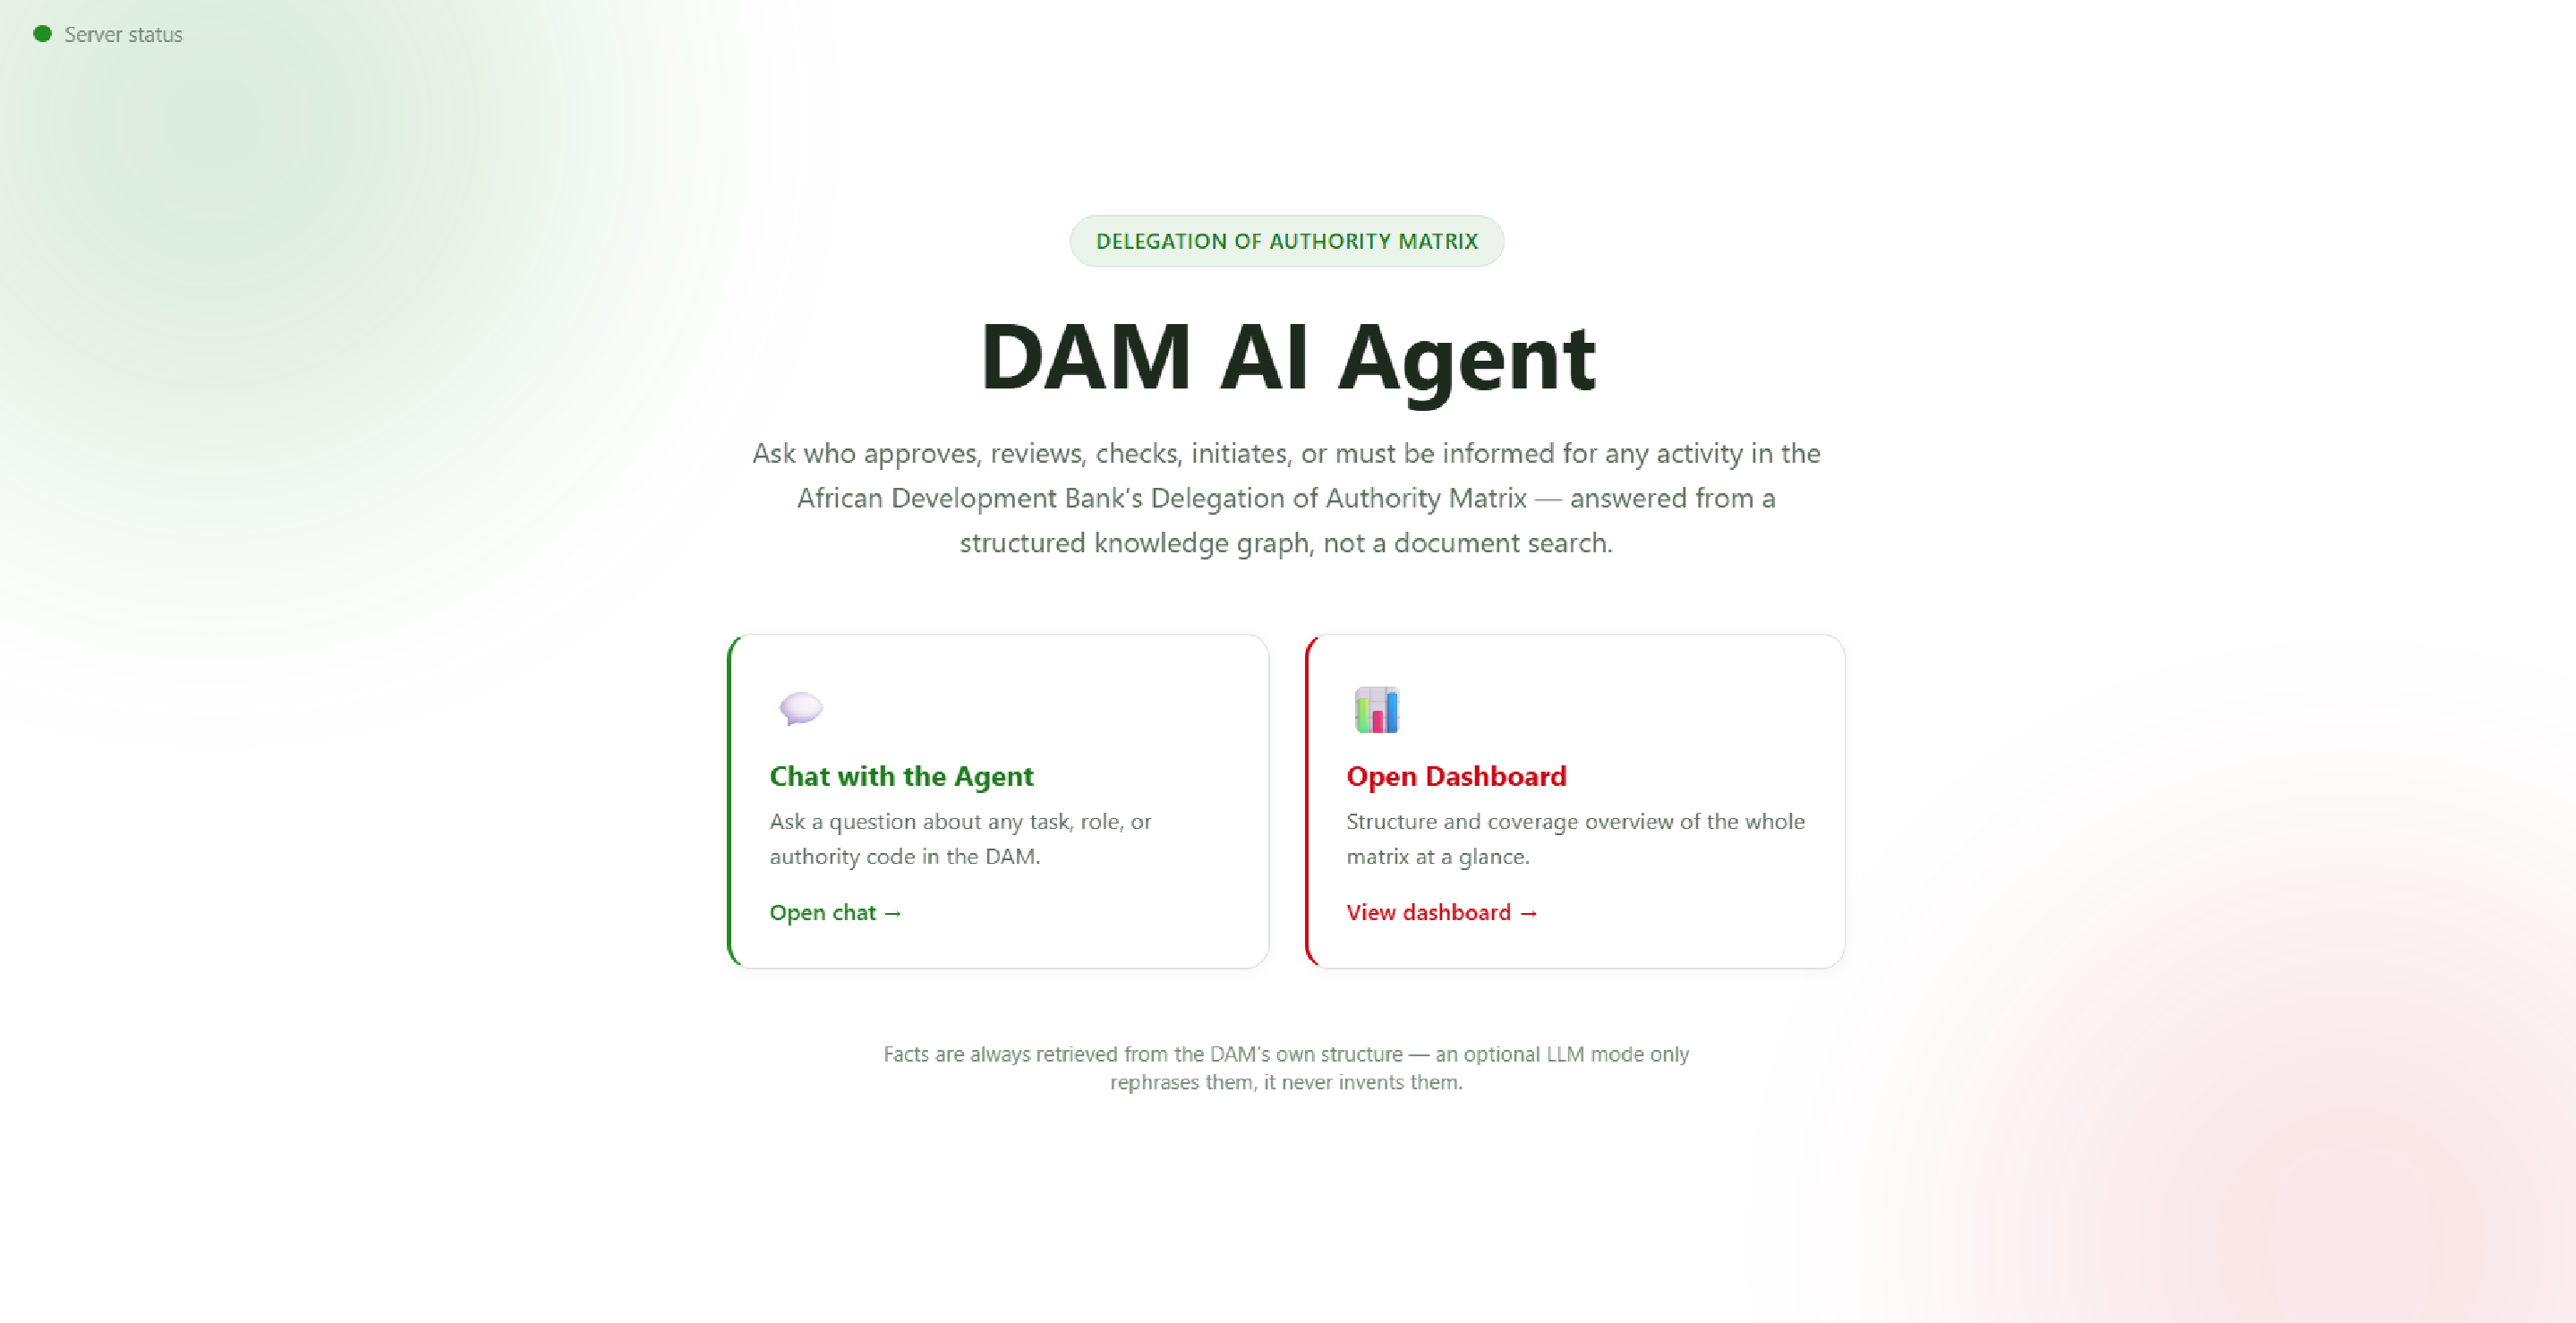
\includegraphics[width=0.96\textwidth]{figures/app-landing.pdf}
\caption{Landing page, which states the grounding guarantee before any question is
asked.}
\label{fig:applanding}
\end{figure}

\subsection{Voice Input}

A question may be dictated instead of typed. The composer exposes a microphone control
which captures audio in the browser through the \texttt{MediaRecorder} interface and posts
the resulting clip to a transcription endpoint, where it is transcribed by a hosted
Whisper model and returned as text. Transcription is therefore server-mediated rather than
performed in the browser, which keeps behaviour identical across browsers that implement
on-device speech recognition inconsistently or not at all.

One design decision is deliberate and easy to miss. The returned transcript is placed into
the input field for review rather than submitted automatically. Speech recognition
performs poorly on institutional acronyms and on numeric activity identifiers, which is
exactly what these questions contain; a user who never sees the transcript cannot correct
an identifier that was misheard. Routing the transcript through the input field also means
it passes through the deterministic typo correction described in
Chapter~\ref{ch:agent} before retrieval, so a near-miss transcription is frequently
recovered without the user intervening at all.

Answers can also be read aloud, and this direction genuinely is browser-local: playback
uses the browser's own speech synthesis interface, selecting a voice matching the answer
language, with no audio leaving the machine.

\subsection{Attachment Question Answering}

A document may be attached to a conversation and questioned directly. The intended use is
a source that is not the DAM: a draft policy, a procedure note, or a revised extract of
the matrix that has not yet been published.

Uploads are constrained by an allowlist rather than a denylist, so an unanticipated file
type is refused rather than silently accepted, and by a fifteen-megabyte ceiling enforced
before any byte reaches the storage layer. Accepted files are stored in an S3-compatible
object bucket under a key namespaced by the uploading account, and are retrieved for
reading through short-lived presigned URLs rather than public links, since a conversation
may be reopened long after the attachment was posted and there is no point at which
minting a permanent URL would be correct.

Answering differs by document type. Text, CSV, PDF and Word documents are reduced to plain
text, PDFs through the same character-level extractor used by the pipeline and Word
documents through a dedicated reader, and the extracted text is supplied to the language
model with an instruction to answer only from that text and to say plainly when the answer
is not present in it. Images are handled through a vision-capable model instead, and the
system establishes that the selected provider supports vision before attempting the
request rather than discovering mid-request that it does not. Formats that cannot be read
reliably, legacy binary Word files and spreadsheets among them, are refused with a message
naming the limitation.

The important property of this feature is not the capability but the boundary it draws.
An answer derived from an attachment is labelled as such in the interface and carries no
activity identifier, because there is none: it did not come from the graph. The guarantee
defended throughout this report is that an answer about the DAM is assembled from a
verified extraction of a verified document. An uploaded file has been through no such
process. It may be a draft, it may be superseded, and the system says so by refusing to
present the two kinds of answer in the same visual language.

\subsection{Interface Localisation}

The agent answers in five languages. The conversation interface follows: its controls, its
placeholder text, its empty state, and the provenance labels beneath each answer are held
in a message catalogue with one entry set per supported language, and a missing entry
falls back to English rather than rendering a raw key. For Arabic the document direction
is set to right-to-left so that the conversation layout mirrors correctly.

The scope is the conversation interface, and it is worth being precise rather than
generous about that: the landing page, the sign-in form, and the dashboard remain in
English. Extending the catalogue to those surfaces is mechanical rather than difficult,
and is recorded here as incomplete rather than described as done.

One category of text is deliberately never translated. Role names, activity titles,
authority codes and identifiers are reproduced exactly as the source document records
them, in every language. They are content rather than interface text, and translating them
would break both the traceability requirement and the verification mechanism of
Chapter~\ref{ch:agent}, which matches generated text against the literal role names held
in the graph.

\section{Conversation Persistence and Sharing}

Once a conversation belongs to someone, two further questions follow naturally: can it
survive between sessions, and can it be shown to someone else without handing them the
underlying account. The second question is where the real-time mechanism that keeps a
shared view from silently going stale comes in.

\subsection{Conversations as Owned Objects}

Every conversation is persisted server-side against the account that created it, which is
what makes the rest of this section possible: a conversation that exists only in a browser
tab can be neither resumed nor shared. Each exchange is stored with its question, its
answer, and the provenance metadata that accompanied the answer, so a conversation
reopened weeks later carries the same resolution method and confidence score it displayed
originally.

\subsection{Granting Access to a Colleague}

A conversation can be shared with a named colleague, which records a grant against that
account and causes the conversation to appear in their own list. Access is read-only: a
recipient sees the questions, the answers and the provenance, and can add nothing.

\subsection{Link and QR-Code Sharing}

Naming a colleague requires knowing which account they hold, which is an obstacle when the
conversation is being shown to someone standing in the room. The system therefore also
issues a share link: a random token with a seven-day default expiry, rendered by the
client as a QR code so that it can be scanned from a phone without anything being retyped.
Figure~\ref{fig:appshare} shows the share dialogue with a generated code.

\begin{figure}[htbp]
\centering
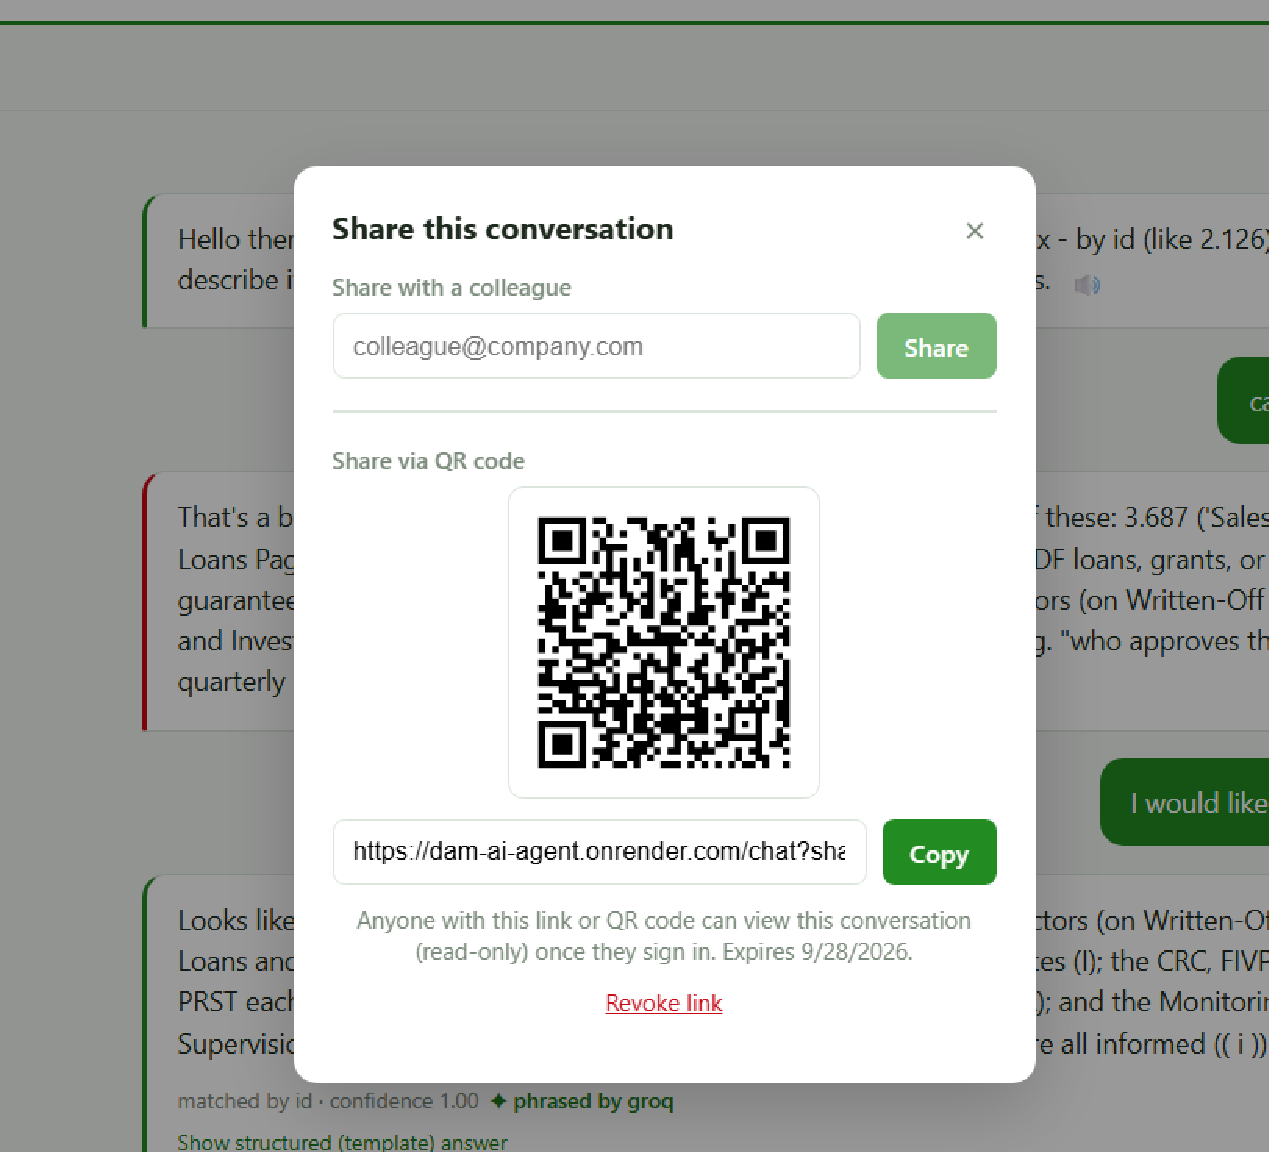
\includegraphics[width=0.7\textwidth]{figures/app-share-qr.pdf}
\caption{Sharing dialogue. A conversation may be shared with a named colleague or
through an expiring link rendered as a QR code, with the expiry date stated and revocation
available.}
\label{fig:appshare}
\end{figure}

Visiting a share link does not itself grant access. The recipient must be signed in, and
claiming the link invokes the same grant used by direct sharing, so the question of who
may view a conversation has exactly one answer in the code rather than two that must be
kept consistent. A link that has expired or been revoked is refused; the originating user
may revoke at any time before expiry.

\subsection{Real-Time Propagation}

A shared conversation is a live view rather than a copy. Messages added after sharing
appear to the recipient, which is the behaviour a colleague consulted mid-conversation
expects, and which a snapshot cannot provide.

Propagation uses two mechanisms together. The server maintains a per-account publish and
subscribe registry and pushes events to connected clients over a Server-Sent Events stream,
so a new message typically reaches a shared viewer within about a second. A thirty-second
poll runs alongside it. The redundancy is intentional: the stream is a long-lived
connection and free hosting tiers are not reliable custodians of those, so the poll bounds
how stale a view can become if the stream is dropped silently. One implementation detail
proved necessary in practice, namely that a background refresh is never permitted to
shorten a conversation already on screen, which otherwise allowed a poll completing
between a message being sent and its response arriving to momentarily erase it from the
sender's own view.

The registry is per-process, which is correct for the single-instance deployment described
later in this chapter and would require a shared broker to survive horizontal scaling.
This is recorded as a known boundary rather than left to be discovered.

Figure~\ref{fig:sharesse} traces one message through both channels, and the rule at the
bottom of the diagram is the one implementation detail mentioned above: a background
refresh may add messages to a shared view but may never remove or shorten what is already
displayed.

\begin{figure}[htbp]
\centering
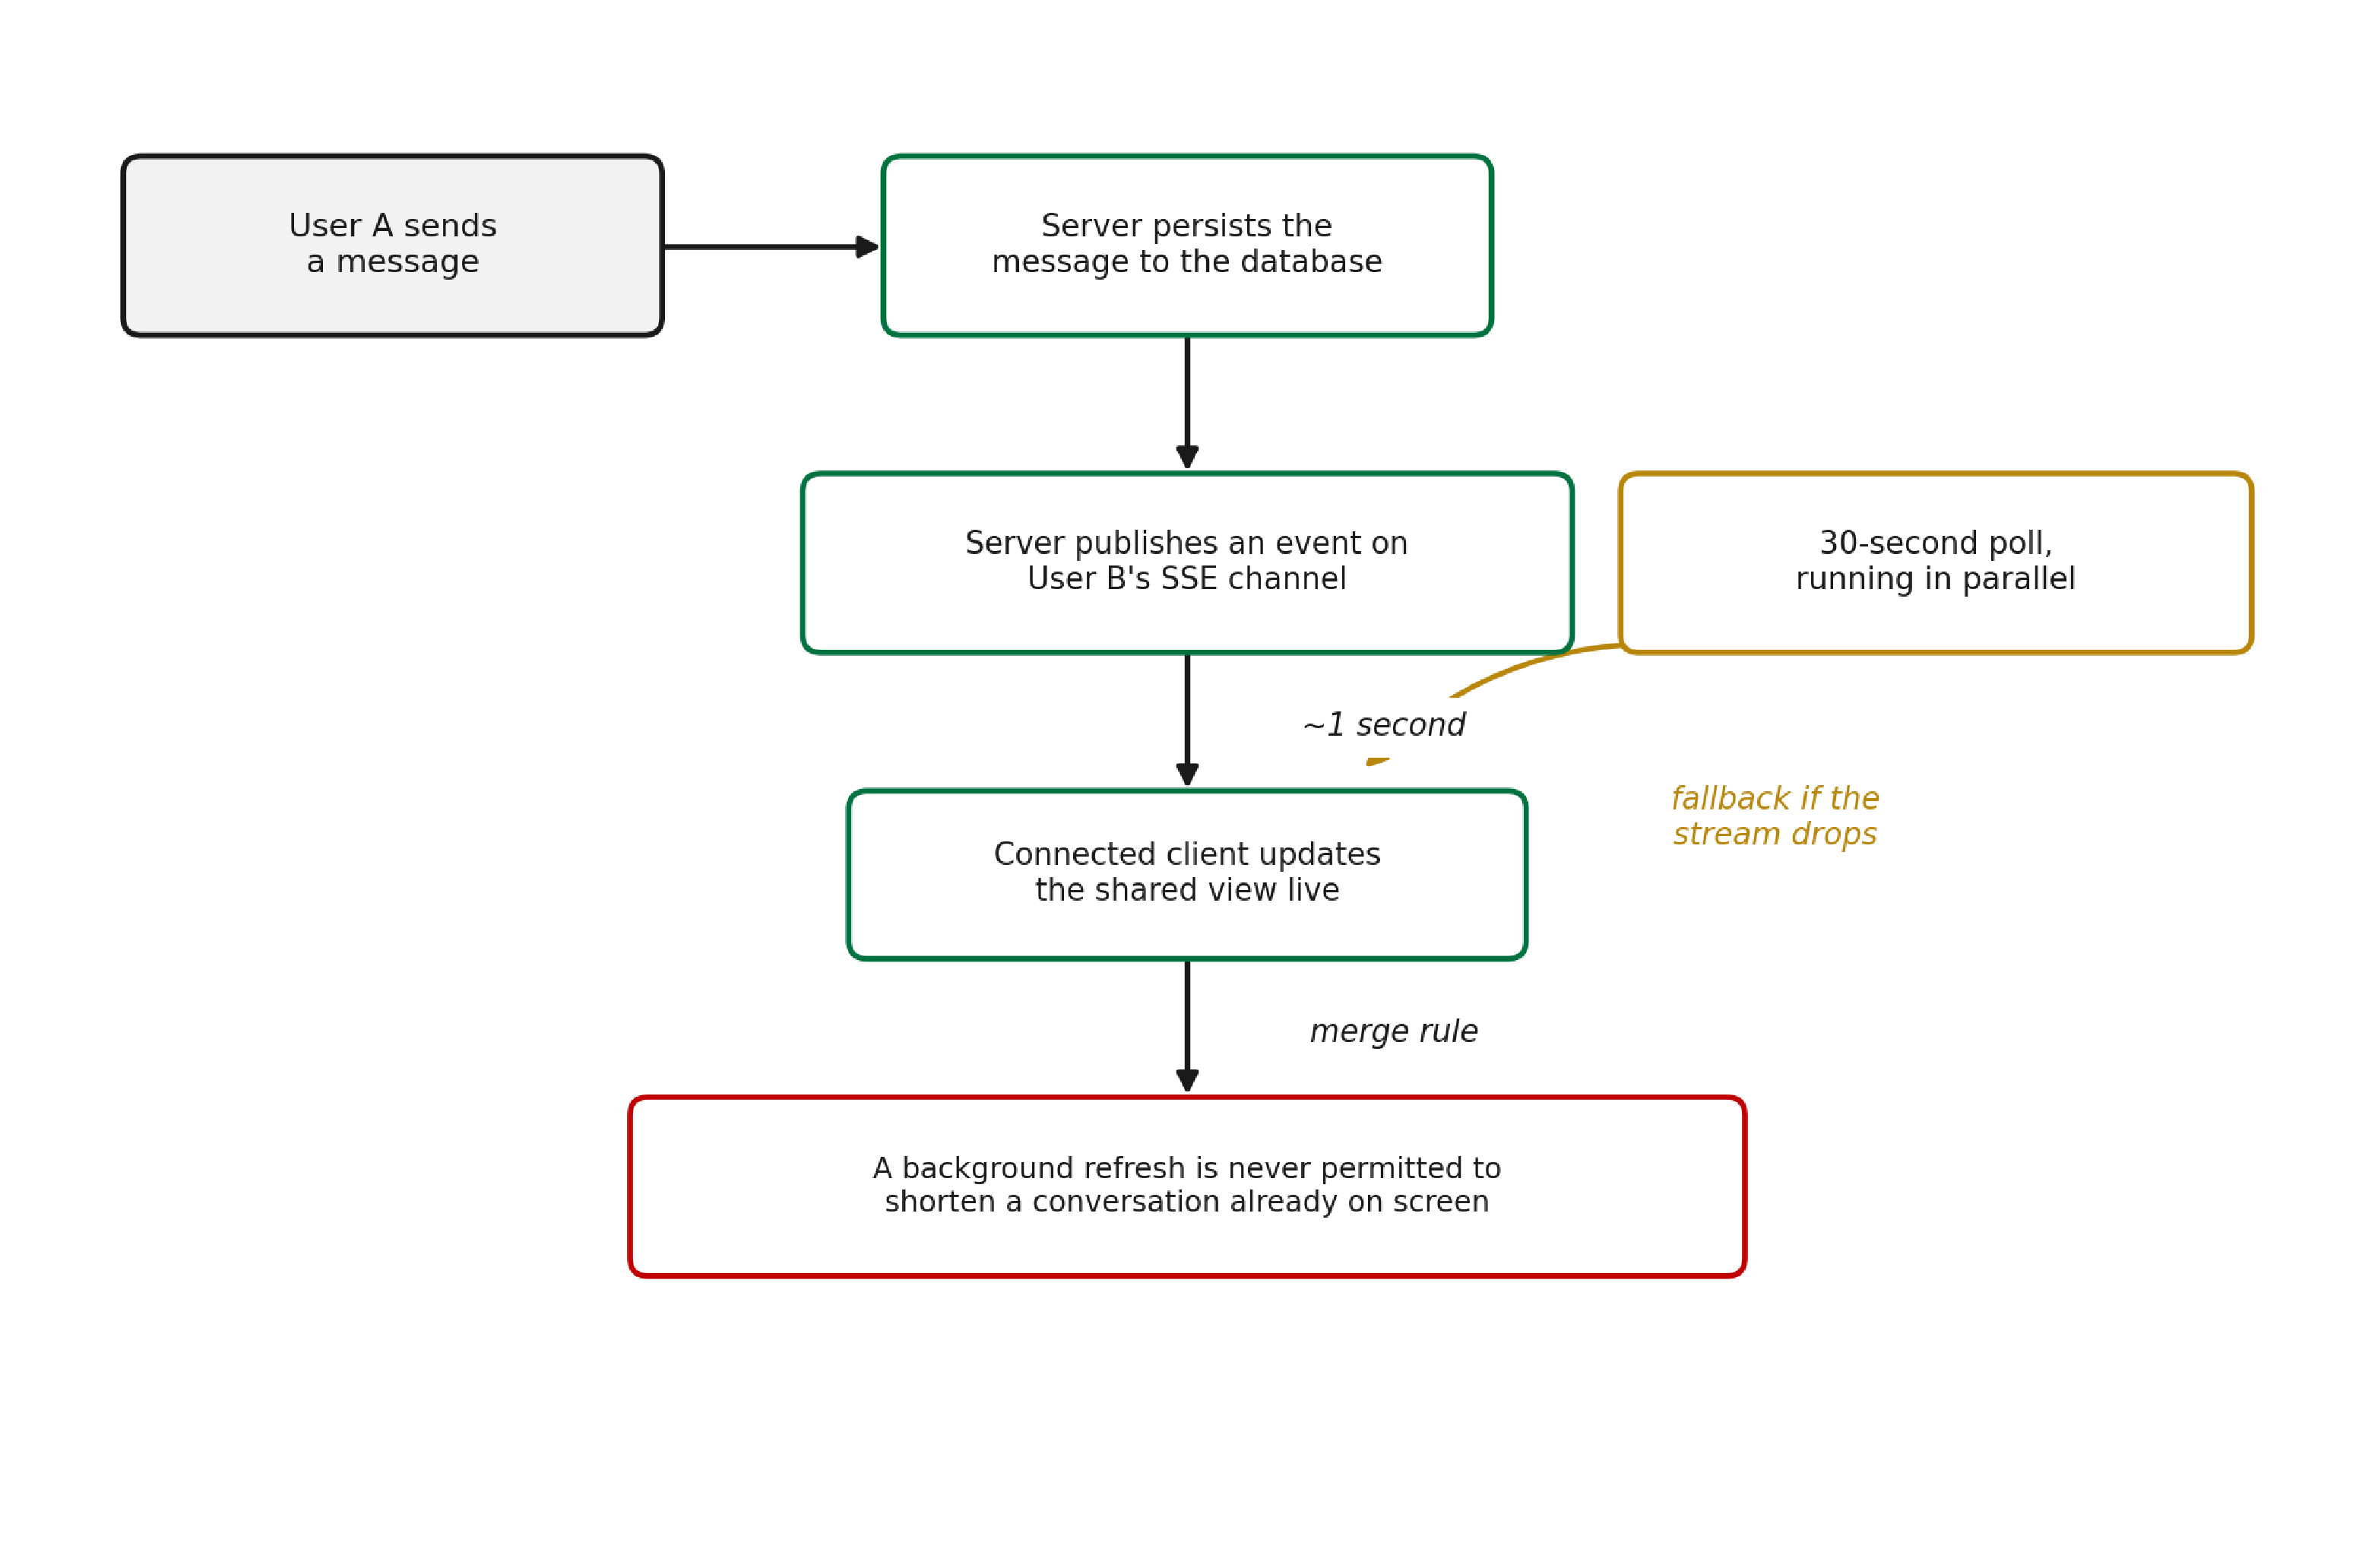
\includegraphics[width=0.86\textwidth]{figures/fig-sharesse.pdf}
\caption{Real-time propagation of a shared conversation. The Server-Sent Events stream
delivers a new message within about a second; the thirty-second poll is a fallback that
bounds staleness if the stream drops.}
\label{fig:sharesse}
\end{figure}

\section{Analytics Dashboard}

Everything up to this point has been about answering a question against one activity at a
time. The dashboard is the platform's one departure from that pattern: why it exists, how
its numbers are computed, which indicators earned a place on it, and which governance
indicators were specified but held back from the delivered release.

\subsection{Purpose}

Every other part of the platform answers questions about individual activities. The
dashboard does something different: it reports on the matrix as an object, and in doing so
exposes properties that no page-by-page reading reveals. A reader consulting the document
sees one activity at a time by construction. Questions such as how many roles hold
approval authority at all, how concentrated that authority is, or what proportion of the
document carries no responsibilities of its own, cannot be answered by reading. They can
be answered immediately once the same document is a graph.

Figure~\ref{fig:appdashboard} shows the delivered dashboard.

\begin{figure}[htbp]
\centering
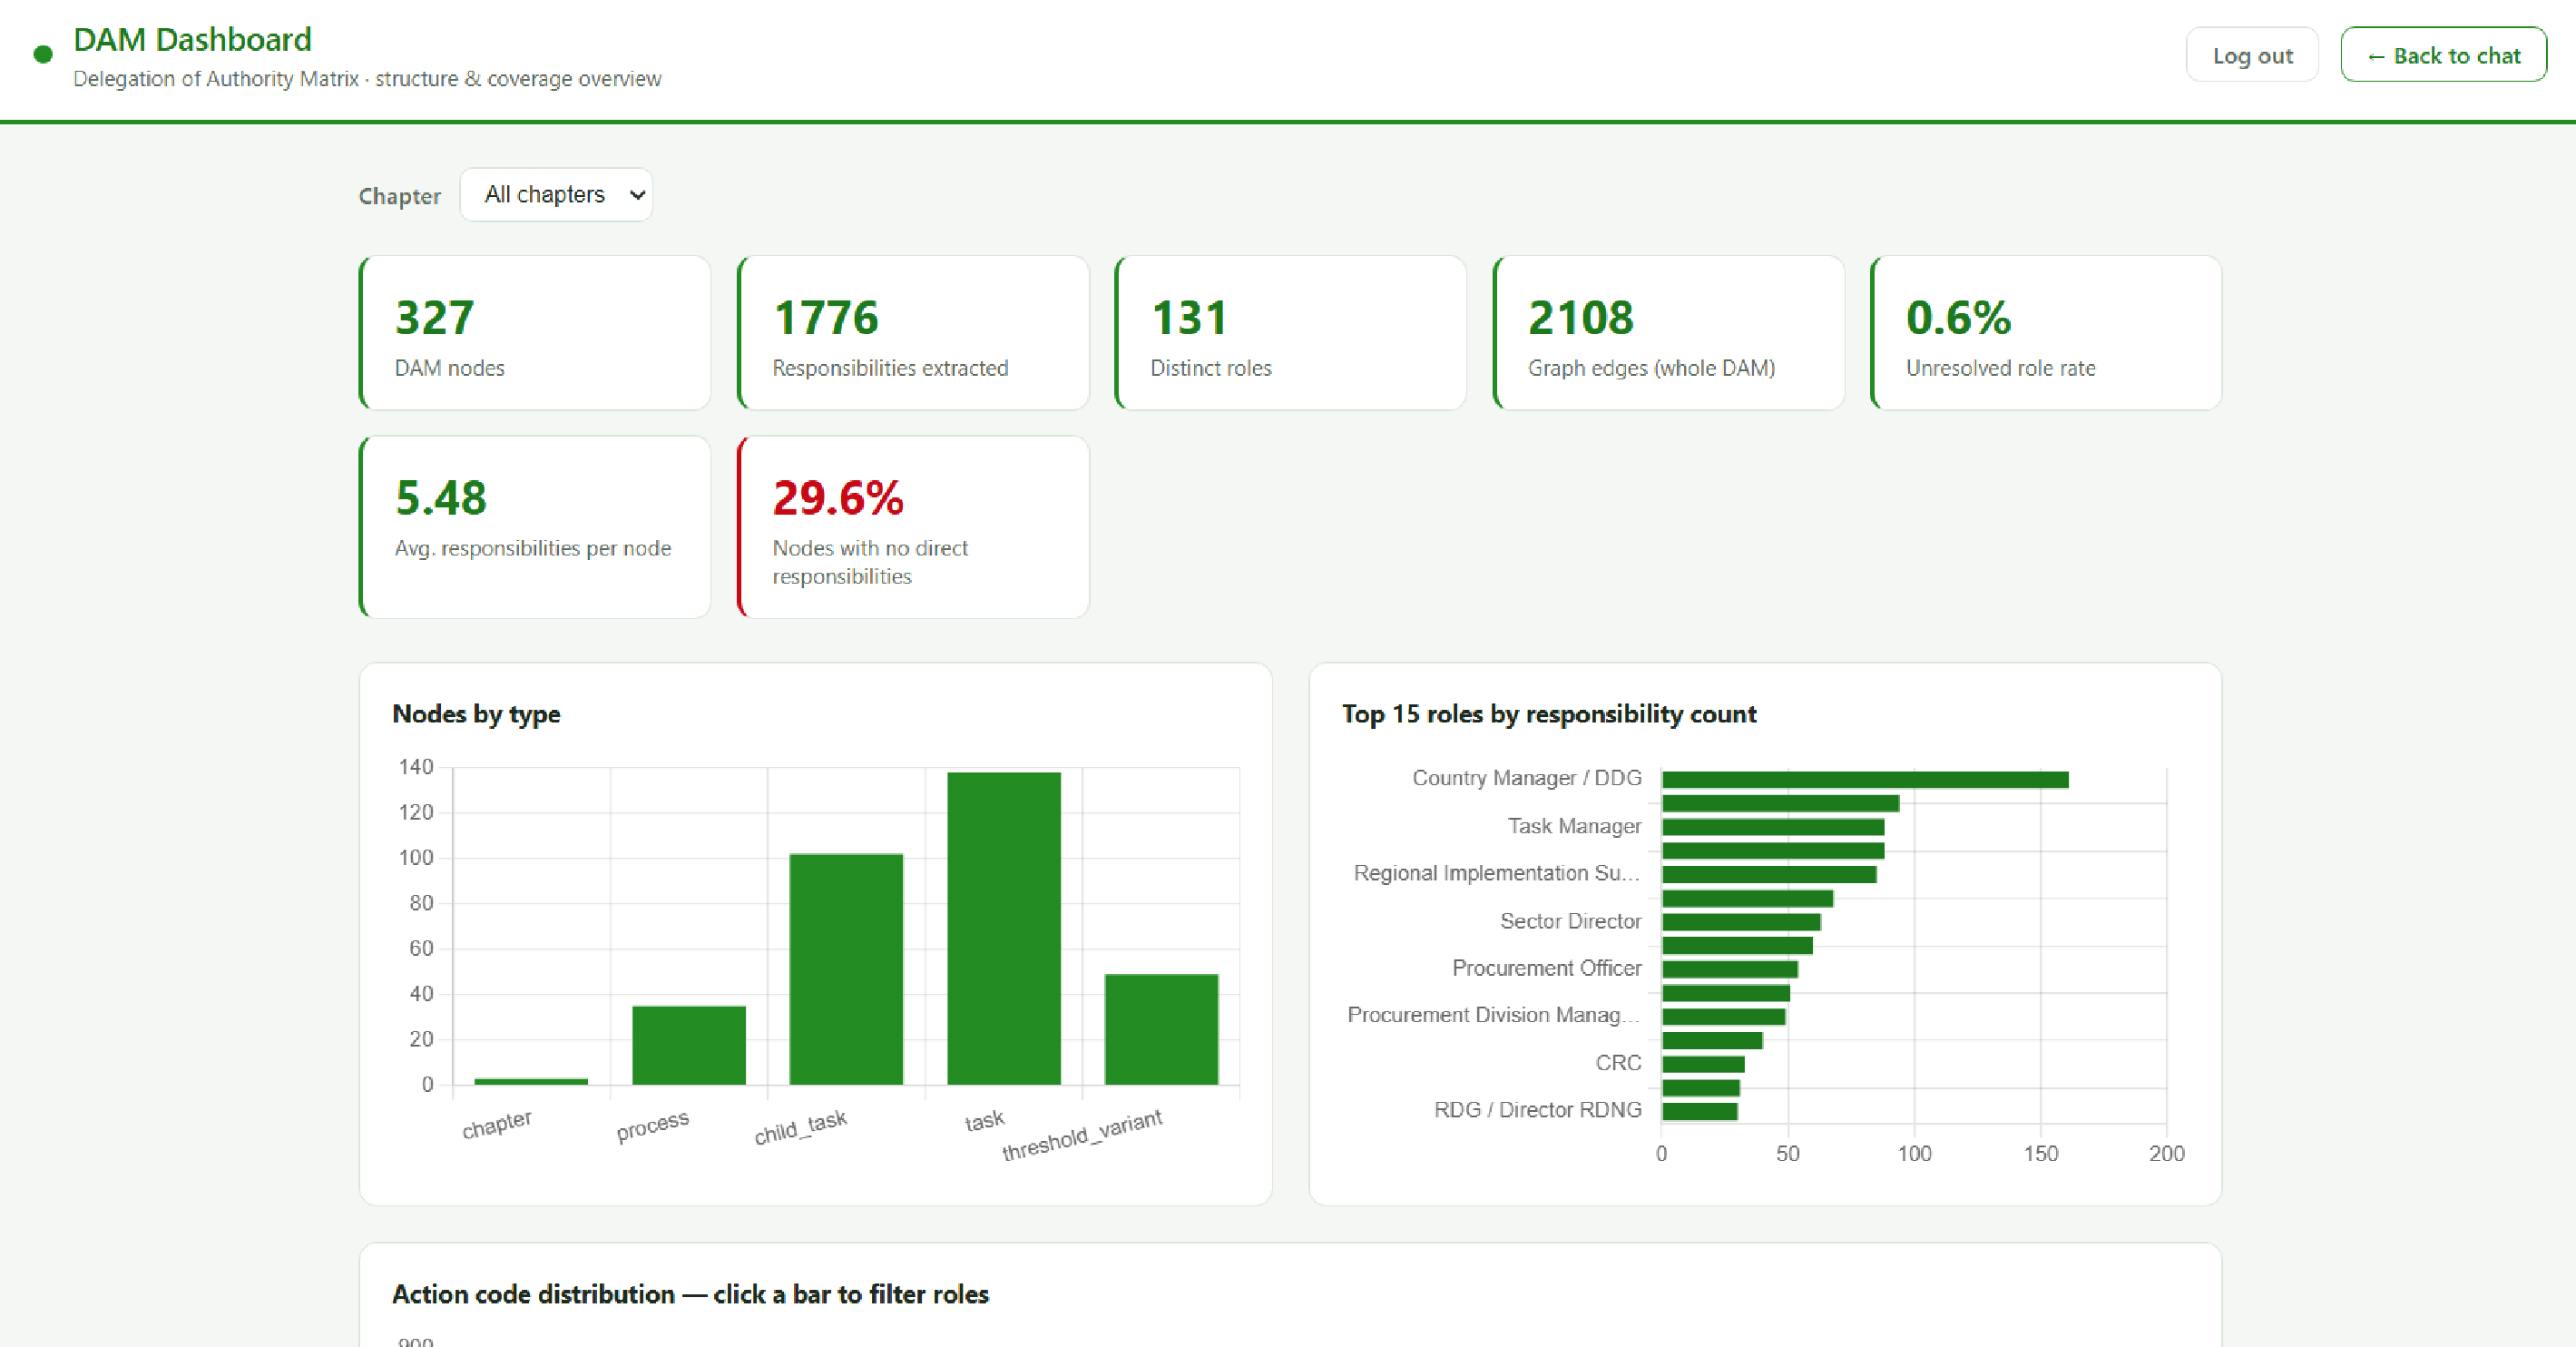
\includegraphics[width=0.98\textwidth]{figures/app-dashboard.pdf}
\caption{Analytics dashboard, showing headline indicators, the distribution of node
types, and the roles ranked by the number of responsibilities they carry.}
\label{fig:appdashboard}
\end{figure}

\subsection{Computation Model}

No statistic on the dashboard is stored. Every figure is computed at request time from the
node set and the graph already held in memory, which has one consequence worth stating
explicitly: the dashboard cannot drift out of agreement with the knowledge base, because
there is no second copy of the numbers that could become stale. A parser change that
alters the extraction is visible on the dashboard at the next request without any
recomputation step, and the cost of that guarantee is an aggregation over a few hundred
nodes, which is negligible.

The same computation is applied twice at different scopes. It runs once over every node in
the matrix, and once per chapter over that chapter's nodes, producing an identical
structure in both cases so that the client can render the whole-document view and a
single-chapter view through the same code path.

One quantity is deliberately not scoped by chapter. The graph edge total remains
whole-document, because responsibility and cross-reference edges routinely cross chapter
boundaries: the same role appears in several chapters, and a reference in one chapter
frequently points into another. A per-chapter edge count would require a defensible rule
for whether an edge leaving the chapter belongs to it, and any such rule would produce a
number more misleading than useful.

\subsection{How Indicators Were Chosen}

An indicator earns its place on a dashboard by changing what somebody does. That criterion
is easy to state and routinely ignored, and the usual result is a wall of counts that is
read once out of curiosity and never again. Each figure reported here was therefore required
to answer a specific question that somebody actually has, and the indicators fall into three
groups according to whose question it is.

The first group answers \emph{is the extraction still correct}, and its audience is whoever
maintains the pipeline. These are regression instruments: they exist because a parser change
can break a rule silently, producing a node set that is smaller or emptier or differently
distributed while every individual record still looks plausible. A sampled manual check does
not catch that. A number that moves does.

The second group answers \emph{what is in this document}, and its audience is a reader
trying to understand the matrix as an object rather than to look one activity up. A person
consulting the DAM sees one activity at a time by construction, which makes the shape of the
whole invisible to them however carefully they read.

The third group answers \emph{what does this document imply about the institution}, and its
audience is governance and audit. These are the indicators of Section~\ref{sec:govkpi}, and
they are specified rather than delivered.

The rest of this section takes the delivered indicators in turn and states, for each, what it
measures, why it was chosen, and what it turned out to show. Table~\ref{tab:dashkpi}
summarises them first.

\begin{longtable}{|p{0.27\textwidth}|p{0.11\textwidth}|p{0.14\textwidth}|p{0.36\textwidth}|}
\caption{Indicators computed by the delivered analytics dashboard.}\label{tab:dashkpi}\\
\hline
\rowcolor{myblue}\textcolor{white}{\textbf{Indicator}} & \textcolor{white}{\textbf{Value}} & \textcolor{white}{\textbf{Answers}} & \textcolor{white}{\textbf{Why it is reported}} \\
\hline
\endfirsthead
\hline
\rowcolor{myblue}\textcolor{white}{\textbf{Indicator}} & \textcolor{white}{\textbf{Value}} & \textcolor{white}{\textbf{Answers}} & \textcolor{white}{\textbf{Why it is reported}} \\
\hline
\endhead
DAM nodes & 327 & What is in it & Establishes the size of the extracted corpus and moves immediately if a parsing change drops records. \\ \hline
Responsibilities extracted & 1{,}776 & What is in it & The real size of the matrix. Activities are containers; obligations are the content. \\ \hline
Distinct roles & 131 & What is in it & Bounds how many organisational actors the delegation structure involves at all. \\ \hline
Graph edges & 2{,}108 & What is in it & Confirms the graph is connected rather than a set of isolated records. \\ \hline
Unresolved role rate & 0.6\% & Is it correct & The single most sensitive regression detector in the project. \\ \hline
Average responsibilities per node & 5.48 & What is in it & Procedural weight per activity, and a second regression signal. \\ \hline
Nodes with no direct responsibilities & 29.6\% & What is in it & Quantifies the redirect structure, and justifies a correctness requirement of the agent. \\ \hline
Node type distribution & --- & What is in it & Separates structural scaffolding from actionable activity. \\ \hline
Authority code distribution & --- & What is in it & Shows which obligations the institution actually uses, against the seventeen available. \\ \hline
Top roles by responsibility count & --- & What is in it & Ranks actors by load and exposes concentration. \\ \hline
\end{longtable}

\subsection{Correctness Indicators}

\paragraph{Unresolved role rate.} This measures the proportion of responsibilities whose
authority code was located in a cell but whose owning column could not be determined. It
exists because of how role attribution works: column headers in the source are printed
rotated through ninety degrees, are not recoverable as table headers, and must be
reconstructed by clustering header coordinates and matching each code to a column by
horizontal alignment. That reconstruction is the most fragile step in the pipeline, and when
it degrades it does so quietly, attaching obligations to no role at all rather than raising
an error.

It was added as a development instrument rather than as an analytical one. During the
geometric attribution work it was the number watched after every change, because a
modification that improved one page's clustering while breaking another's is invisible in a
sampled check and unmistakable here. Its present value of 0.6\% is the figure against which
the pipeline's adequacy is argued in Chapter~\ref{ch:pipeline}, and the ten or so
responsibilities behind that percentage are the residue of genuinely ambiguous layout rather
than a systematic fault.

\paragraph{Average responsibilities per node.} At 5.48, this serves a similar purpose from
the opposite direction. The unresolved rate catches codes that lost their role; this catches
codes that were never found. A parsing change that stops recognising a code in some layout
leaves every remaining record perfectly valid, so nothing fails, and the only symptom is that
activities become quietly thinner. Watching a mean rather than a total matters here, because
a total also moves when the processed scope changes, and a ratio does not.

\subsection{Structural Indicators}

\paragraph{Node and responsibility counts.} The corpus contains 327 records carrying 1,776
individual responsibilities. Reporting both is deliberate, because the second is the real
measure of the matrix and the first is routinely mistaken for it. An activity is a container;
the obligations attached to it are the content, and a document with few activities and many
obligations each is a very different thing from the reverse.

\paragraph{Node type distribution.} Records are counted by type, which separates the document
into structural scaffolding and actionable content. Chapters and processes exist to organise;
tasks, child tasks and threshold variants are what a user actually asks about. The
distribution is what makes it possible to say honestly how much of a 79-page document is
answerable material rather than hierarchy, and it also exposes the threshold-variant
population, which is the mechanism behind the near-identical-activities problem that motivated
the whole project in Chapter~\ref{ch:context}.

\paragraph{Authority code distribution.} Seventeen level-qualified notations are available in
the legend. This indicator shows which of them the institution actually uses and how often,
and the interesting result is the imbalance: the delegation structure leans heavily on a
small subset, while several codes appear rarely enough that their meaning is unlikely to be
familiar to most staff. That is an argument for the glossary expansion built into the agent,
grounded in a measurement rather than an assumption.

\paragraph{Distinct roles and the role ranking.} There are 131 distinct roles, and the top
fifteen by obligation count are ranked. The count bounds the size of the delegation structure;
the ranking exposes its shape. A long flat ranking would indicate authority spread evenly, and
a steep one indicates concentration in a handful of offices. The delivered ranking is visibly
steep, which is the observation that motivates the authority-concentration indicator specified
in Section~\ref{sec:govkpi}.

\paragraph{Graph edges.} The 2,108 edges confirm that the extraction produced a connected
structure rather than a pile of independent records. It is reported because the difference
between a list and a graph is the entire premise of the approach: if containment and reference
edges were absent, the cross-reference following of Chapter~\ref{ch:agent} would have nothing
to traverse.

\subsection{An Indicator That Changed the Design}

\paragraph{Records with no direct responsibilities.} At 29.6\%, this is the figure with the
largest consequence in the chapter, and it was not anticipated.

It counts responsibility-bearing records that carry no obligation of their own. Encountering
it for the first time, the natural reading is that something is broken: nearly a third of the
extracted activities appear empty. Checking those records against the printed pages showed the
extraction was correct and the document is simply built that way. Roughly three activities in
ten record nothing themselves and point to another activity instead.

That reframed a feature as a requirement. Cross-reference following had been treated as a
refinement, worth having for completeness. This measurement showed that a system without it
dead-ends on close to a third of the matrix, which is not a gap in polish but a failure on
routine questions. The redirect path described in Chapter~\ref{ch:agent} exists in the form it
does because this number was measured before the agent was finished.

It is also the clearest demonstration of why the dashboard was worth building. The fact was
always present in the document and always invisible to a reader, because a reader
encountering one empty activity concludes that this activity is unusual. Only the aggregate
reveals that it is the norm.

\subsection{Interactive Cross-Filtering}

The charts are linked rather than independent. Selecting an authority code in the
distribution chart filters the role ranking to the roles holding that specific authority,
which turns a static display into a means of asking a different class of question: not
which roles are busiest overall, but which roles hold approval authority specifically, or
which hold check-and-verify obligations. The two rankings are not the same, and the
difference between them is exactly the segregation-of-duties structure of the institution.

The cross-filter is computed server-side rather than derived in the browser, so that the
counting rules, in particular the exclusion of unresolved roles, are applied in one place
and cannot diverge between the ranking and the filtered ranking.

\subsection{Governance Indicators Derivable from the Graph}
\label{sec:govkpi}

The indicators above describe the document. A further family describes what the document
implies about the institution, and the graph supports all of them without requiring any
data source beyond the matrix itself. Table~\ref{tab:govkpi} specifies them.

These are specified rather than delivered. The dashboard as built reports the structural
indicators of Table~\ref{tab:dashkpi}; the governance family below is the designed
extension, defined here precisely enough to be implemented directly, and is not claimed as
a delivered capability.

\begin{longtable}{|p{0.28\textwidth}|p{0.58\textwidth}|}
\caption{Governance indicators derivable from the knowledge graph, specified as the designed extension to the dashboard.}\label{tab:govkpi}\\
\hline
\rowcolor{myblue}\textcolor{white}{\textbf{Indicator}} & \textcolor{white}{\textbf{Definition and interpretation}} \\
\hline
\endfirsthead
\hline
\rowcolor{myblue}\textcolor{white}{\textbf{Indicator}} & \textcolor{white}{\textbf{Definition and interpretation}} \\
\hline
\endhead
Authority concentration & Share of activities for which exactly one role holds approval authority. A high value identifies single points of failure, where one absence blocks a process. \\ \hline
Approval span per role & Number of activities each role approves. Ranks roles by the breadth of authority they carry and surfaces disproportionate concentration. \\ \hline
Segregation of duties & Share of activities where the initiating role differs from the approving role. A standard internal-control measure\citep{coso2013}, computed here directly from the matrix. \\ \hline
Verification coverage & Share of activities carrying at least one recorded check-and-verify obligation. Measures how much of the Bank's activity has a mandatory second pair of eyes. \\ \hline
Notification breadth & Mean number of informed parties per activity, with distribution. Indicates how widely decisions are communicated. \\ \hline
Threshold banding rate & Share of activities whose approver depends on a monetary band. Quantifies how far delegation is value-sensitive rather than flat. \\ \hline
Authority chain depth & Mean number of distinct roles involved in an activity across all authority types. A proxy for procedural weight. \\ \hline
Documentation completeness & Share of activities with no recorded responsibility of any kind, excluding structural containers. Flags gaps in the matrix itself. \\ \hline
Redirect dependency & Share of activities whose responsibilities are reachable only by following a cross-reference. Measures how much of the document is indirect. \\ \hline
Role redundancy & Share of activities with two or more roles able to approve. Read together with authority concentration, it separates resilience from ambiguity. \\ \hline
\end{longtable}

Two of these must be read together rather than separately. Authority concentration and
role redundancy are complementary, and either one alone supports the wrong conclusion: a
single approver is efficient but fragile, while multiple approvers are resilient but can
obscure who is actually accountable. Reported per chapter, the pair shows which pattern
each part of the institution has adopted.

Segregation of duties is the indicator most likely to interest an audit function. It is a
control principle the matrix already implements implicitly, in that the initiating and
approving roles for an activity are recorded separately, and which is currently measured
nowhere. Computing it requires no new data, only the graph that already exists, and it is
the strongest argument in this project for treating a governance document as structured
data rather than as a document.

\section{REST Interface}

Table~\ref{tab:api} lists the endpoints the backend exposes. The surface is deliberately
small, and one property of it is worth noting: the question endpoint is the only route
that reaches the agent, so every path through which an answer can be obtained passes
through the same verification.

\begin{longtable}{|p{0.47\textwidth}|p{0.09\textwidth}|p{0.38\textwidth}|}
\caption{REST API endpoints exposed by the backend.}\label{tab:api}\\
\hline
\rowcolor{myblue}\textcolor{white}{\textbf{Endpoint}} & \textcolor{white}{\textbf{Method}} & \textcolor{white}{\textbf{Purpose}} \\
\hline
\endfirsthead
\hline
\rowcolor{myblue}\textcolor{white}{\textbf{Endpoint}} & \textcolor{white}{\textbf{Method}} & \textcolor{white}{\textbf{Purpose}} \\
\hline
\endhead
\texttt{/api/auth/signup} & POST & Creates an account and returns a signed token. \\ \hline
\texttt{/api/auth/login} & POST & Exchanges credentials for a signed token. Rate-limited. \\ \hline
\texttt{/api/auth/me} & GET & Returns the authenticated account and its role. \\ \hline
\texttt{/api/auth/google/login}, \texttt{/callback} & GET & Federated sign-in through Google. \\ \hline
\texttt{/api/auth/microsoft/login}, \texttt{/callback} & GET & Federated sign-in through Microsoft. \\ \hline
\texttt{/api/ask} & POST & Core endpoint. Accepts a question, model mode, optional carried-over activity, target language, and optional attachment reference. Returns the answer, the deterministic answer, the resolved identifier, resolution method and score, and language and model metadata. \\ \hline
\texttt{/api/uploads} & POST & Stores an attachment against the calling account after type and size validation. \\ \hline
\texttt{/api/transcribe} & POST & Transcribes a dictated audio clip to text. \\ \hline
\texttt{/api/conversations} & GET, POST & Lists owned and shared conversations; creates a conversation. \\ \hline
\texttt{/api/conversations/\{id\}} & GET, DELETE & Retrieves or deletes a conversation. \\ \hline
\texttt{/api/conversations/\{id\}/messages} & POST & Appends an exchange with its provenance metadata. \\ \hline
\texttt{/api/conversations/\{id\}/attachments/\{key\}} & GET & Returns a short-lived presigned URL, subject to conversation-scoped permission. \\ \hline
\texttt{/api/conversations/\{id\}/share} & POST & Grants a named account read-only access. \\ \hline
\texttt{/api/conversations/\{id\}/share/\{user\}} & DELETE & Withdraws a previously granted access. \\ \hline
\texttt{/api/conversations/\{id\}/share-link} & POST, DELETE & Issues or revokes an expiring share link and its QR encoding. \\ \hline
\texttt{/api/conversations/shared/\{token\}/claim} & POST & Claims a share link for the signed-in account. \\ \hline
\texttt{/api/events} & GET & Server-Sent Events stream carrying conversation updates for the authenticated account. \\ \hline
\texttt{/api/dashboard/summary} & GET & Aggregate statistics, per-chapter breakdowns, and graph totals. Administrator only. \\ \hline
\texttt{/api/llm/config} & GET & Reports the model each mode would currently use. \\ \hline
\texttt{/api/health} & GET & Liveness check used by the platform and the status indicator. Reports nodes loaded. \\ \hline
\end{longtable}

\section{Testing and Validation}

The system carries 375 automated tests across 33 files. The count matters less than their
provenance: these are not tests written to reach a coverage target. Almost every one exists
because a specific defect was found, and the test was written to pin the corrected
behaviour so that it could not silently return. Table~\ref{tab:tests} gives the
distribution.

\begin{longtable}{|p{0.34\textwidth}|p{0.09\textwidth}|p{0.45\textwidth}|}
\caption{Breakdown of the automated test suite.}\label{tab:tests}\\
\hline
\rowcolor{myblue}\textcolor{white}{\textbf{Area}} & \textcolor{white}{\textbf{Tests}} & \textcolor{white}{\textbf{Coverage}} \\
\hline
\endfirsthead
\hline
\rowcolor{myblue}\textcolor{white}{\textbf{Area}} & \textcolor{white}{\textbf{Tests}} & \textcolor{white}{\textbf{Coverage}} \\
\hline
\endhead
Extraction and parsing & 42 & Task boundary detection, split-row merging, rotated header extraction, title recovery, reference and footnote handling, glossary parsing \\ \hline
Node and graph construction & 16 & Node assembly, hierarchy correctness, graph edges, lossless caching \\ \hline
Retrieval and agent behaviour & 63 & Identifier fast path, free-text resolution, typo tolerance, small talk, authority codes, glossary lookup, answer orchestration \\ \hline
Language model layer & 59 & Provider mocking and failure handling, verification-step correctness, translation, tone classification \\ \hline
Attachments and storage & 37 & Text extraction per format, vision routing, object storage, upload validation, attachment question answering \\ \hline
Authentication and accounts & 21 & Password hashing, token issuance and expiry, rate limiting, federated sign-in \\ \hline
Conversations and sharing & 33 & Persistence, direct shares, share links, claim, expiry, revocation \\ \hline
Real-time events & 6 & Publish and subscribe registry, fan-out, de-duplication \\ \hline
API and error handling & 42 & End-to-end route behaviour, attachment branch authorisation, unhandled-error contract \\ \hline
Dashboard and client & 31 & Dashboard metrics, chapter scoping, structural checks on the web client source \\ \hline
\textbf{Total} & \textbf{375} & \textbf{across 33 files} \\ \hline
\end{longtable}

Automated testing was not the only form of verification. Individual records were checked
against the printed pages they were extracted from, which is the only way to detect an
answer that is plausible and wrong, and the running system was exercised with real
questions before each significant change.

Two defects found during a late verification pass are reported here rather than removed. In
one pair of records a column header was attributed as though it were a role, producing a
responsibility held by a role name that does not exist in the organisation. In the same two
records, two adjacent footnote digits were fused into a single number, yielding a footnote
reference that matches no actual footnote. Both are localised to those records, both are
visible in a live answer, and both are scheduled for correction alongside the footnote
extraction work described in the general conclusion. They are stated because a report that
describes only the defects that were fixed gives a misleading account of the state of the
system.

\section{Deployment}
\label{sec:deployment}

The application is containerised\citep{docker_docs} through a multi-stage build that
compiles the web client and packages the result with the Python service, so the image that
runs in production is the image that was built and tested rather than an environment
assembled at deploy time. A companion composition adds a local model container for offline
operation; the hosted provider needs no container, being reached over the network.

Deployment targets a free hosting tier\citep{render_docs} with automatic redeployment on
every change to the main branch. The first attempt failed, and the failure is instructive.
The service parsed the source PDF at startup, exceeded the platform's memory ceiling, and
was terminated before it ever served a request. The resolution was to move parsing to
build time and ship the serialised node set, reducing startup to a file load. This brought
both memory use and startup time within the platform's limits, and it is the direct reason
the knowledge base is an immutable build artefact rather than something constructed at
runtime, as described at the start of this chapter. The constraint produced the
architecture.

\section*{Conclusion}
\addcontentsline{toc}{section}{Conclusion}

This chapter has presented the platform delivered around the agent. Authentication
establishes ownership; ownership makes persistence meaningful; persistence makes sharing
possible; and sharing, once conversations are live objects rather than snapshots,
required a real-time channel. Each capability rests on the one before it, and none of them
required modifying the retrieval or generation components, which is the practical payoff
of the architectural separation argued for in Chapter~\ref{ch:agent}.

The dashboard is the part of the system that does something the original document cannot.
Reading the matrix answers questions about one activity; querying the graph answers
questions about the institution. The structural indicators delivered here are modest in
number, but two of them, the unresolved role rate and the proportion of records with no
direct responsibilities, turned out to serve as both engineering instruments and
analytical findings, the second quantifying a redirect structure that directly justifies a
correctness requirement of the agent.

The system is deployed, reachable, and covered by 375 automated tests. It is also
incomplete in ways this chapter has stated rather than concealed: localisation stops at
the conversation interface, the governance indicators are specified but not implemented,
and two extraction defects remain live. The general conclusion which follows sets these
against what the project set out to do.
